
%% bare_jrnl_compsoc.tex
%% V1.3
%% 2007/01/11
%% by Michael Shell
%% See:
%% http://www.michaelshell.org/
%% for current contact information.
%%
%% This is a skeleton file demonstrating the use of IEEEtran.cls
%% (requires IEEEtran.cls version 1.7 or later) with an IEEE Computer
%% Society journal paper.
%%
%% Support sites:
%% http://www.michaelshell.org/tex/ieeetran/
%% http://www.ctan.org/tex-archive/macros/latex/contrib/IEEEtran/
%% and
%% http://www.ieee.org/

%%*************************************************************************
%% Legal Notice:
%% This code is offered as-is without any warranty either expressed or
%% implied; without even the implied warranty of MERCHANTABILITY or
%% FITNESS FOR A PARTICULAR PURPOSE! 
%% User assumes all risk.
%% In no event shall IEEE or any contributor to this code be liable for
%% any damages or losses, including, but not limited to, incidental,
%% consequential, or any other damages, resulting from the use or misuse
%% of any information contained here.
%%
%% All comments are the opinions of their respective authors and are not
%% necessarily endorsed by the IEEE.
%%
%% This work is distributed under the LaTeX Project Public License (LPPL)
%% ( http://www.latex-project.org/ ) version 1.3, and may be freely used,
%% distributed and modified. A copy of the LPPL, version 1.3, is included
%% in the base LaTeX documentation of all distributions of LaTeX released
%% 2003/12/01 or later.
%% Retain all contribution notices and credits.
%% ** Modified files should be clearly indicated as such, including  **
%% ** renaming them and changing author support contact information. **
%%
%% File list of work: IEEEtran.cls, IEEEtran_HOWTO.pdf, bare_adv.tex,
%%                    bare_conf.tex, bare_jrnl.tex, bare_jrnl_compsoc.tex
%%*************************************************************************

% *** Authors should verify (and, if needed, correct) their LaTeX system  ***
% *** with the testflow diagnostic prior to trusting their LaTeX platform ***
% *** with production work. IEEE's font choices can trigger bugs that do  ***
% *** not appear when using other class files.                            ***
% The testflow support page is at:
% http://www.michaelshell.org/tex/testflow/




% Note that the a4paper option is mainly intended so that authors in
% countries using A4 can easily print to A4 and see how their papers will
% look in print - the typesetting of the document will not typically be
% affected with changes in paper size (but the bottom and side margins will).
% Use the testflow package mentioned above to verify correct handling of
% both paper sizes by the user's LaTeX system.
%
% Also note that the "draftcls" or "draftclsnofoot", not "draft", option
% should be used if it is desired that the figures are to be displayed in
% draft mode.
%
% The Computer Society usually requires 10pt for submissions.
%
\documentclass[10pt,journal,cspaper,compsoc]{IEEEtran}
%
% If IEEEtran.cls has not been installed into the LaTeX system files,
% manually specify the path to it like:
% \documentclass[12pt,journal,compsoc]{../sty/IEEEtran}





% Some very useful LaTeX packages include:
% (uncomment the ones you want to load)


% *** MISC UTILITY PACKAGES ***
%
%\usepackage{ifpdf}
% Heiko Oberdiek's ifpdf.sty is very useful if you need conditional
% compilation based on whether the output is pdf or dvi.
% usage:
% \ifpdf
%   % pdf code
% \else
%   % dvi code
% \fi
% The latest version of ifpdf.sty can be obtained from:
% http://www.ctan.org/tex-archive/macros/latex/contrib/oberdiek/
% Also, note that IEEEtran.cls V1.7 and later provides a builtin
% \ifCLASSINFOpdf conditional that works the same way.
% When switching from latex to pdflatex and vice-versa, the compiler may
% have to be run twice to clear warning/error messages.






% *** CITATION PACKAGES ***
%
\ifCLASSOPTIONcompsoc
  % IEEE Computer Society needs nocompress option
  % requires cite.sty v4.0 or later (November 2003)
  % \usepackage[nocompress]{cite}
\else
  % normal IEEE
  % \usepackage{cite}
\fi
% cite.sty was written by Donald Arseneau
% V1.6 and later of IEEEtran pre-defines the format of the cite.sty package
% \cite{} output to follow that of IEEE. Loading the cite package will
% result in citation numbers being automatically sorted and properly
% "compressed/ranged". e.g., [1], [9], [2], [7], [5], [6] without using
% cite.sty will become [1], [2], [5]--[7], [9] using cite.sty. cite.sty's
% \cite will automatically add leading space, if needed. Use cite.sty's
% noadjust option (cite.sty V3.8 and later) if you want to turn this off.
% cite.sty is already installed on most LaTeX systems. Be sure and use
% version 4.0 (2003-05-27) and later if using hyperref.sty. cite.sty does
% not currently provide for hyperlinked citations.
% The latest version can be obtained at:
% http://www.ctan.org/tex-archive/macros/latex/contrib/cite/
% The documentation is contained in the cite.sty file itself.
%
% Note that some packages require special options to format as the Computer
% Society requires. In particular, Computer Society  papers do not use
% compressed citation ranges as is done in typical IEEE papers
% (e.g., [1]-[4]). Instead, they list every citation separately in order
% (e.g., [1], [2], [3], [4]). To get the latter we need to load the cite
% package with the nocompress option which is supported by cite.sty v4.0
% and later. Note also the use of a CLASSOPTION conditional provided by
% IEEEtran.cls V1.7 and later.





% *** GRAPHICS RELATED PACKAGES ***
%
\ifCLASSINFOpdf
  \usepackage[pdftex]{graphicx}
  % declare the path(s) where your graphic files are
  % \graphicspath{{../pdf/}{../jpeg/}}
  % and their extensions so you won't have to specify these with
  % every instance of \includegraphics
  %\DeclareGraphicsExtensions{.pdf,.jpeg,.png}
\else
  % or other class option (dvipsone, dvipdf, if not using dvips). graphicx
  % will default to the driver specified in the system graphics.cfg if no
  % driver is specified.
  % \usepackage[dvips]{graphicx}
  % declare the path(s) where your graphic files are
  % \graphicspath{{../eps/}}
  % and their extensions so you won't have to specify these with
  % every instance of \includegraphics
  % \DeclareGraphicsExtensions{.eps}
\fi
% graphicx was written by David Carlisle and Sebastian Rahtz. It is
% required if you want graphics, photos, etc. graphicx.sty is already
% installed on most LaTeX systems. The latest version and documentation can
% be obtained at: 
% http://www.ctan.org/tex-archive/macros/latex/required/graphics/
% Another good source of documentation is "Using Imported Graphics in
% LaTeX2e" by Keith Reckdahl which can be found as epslatex.ps or
% epslatex.pdf at: http://www.ctan.org/tex-archive/info/
%
% latex, and pdflatex in dvi mode, support graphics in encapsulated
% postscript (.eps) format. pdflatex in pdf mode supports graphics
% in .pdf, .jpeg, .png and .mps (metapost) formats. Users should ensure
% that all non-photo figures use a vector format (.eps, .pdf, .mps) and
% not a bitmapped formats (.jpeg, .png). IEEE frowns on bitmapped formats
% which can result in "jaggedy"/blurry rendering of lines and letters as
% well as large increases in file sizes.
%
% You can find documentation about the pdfTeX application at:
% http://www.tug.org/applications/pdftex





% *** MATH PACKAGES ***
%
%\usepackage[cmex10]{amsmath}
% A popular package from the American Mathematical Society that provides
% many useful and powerful commands for dealing with mathematics. If using
% it, be sure to load this package with the cmex10 option to ensure that
% only type 1 fonts will utilized at all point sizes. Without this option,
% it is possible that some math symbols, particularly those within
% footnotes, will be rendered in bitmap form which will result in a
% document that can not be IEEE Xplore compliant!
%
% Also, note that the amsmath package sets \interdisplaylinepenalty to 10000
% thus preventing page breaks from occurring within multiline equations. Use:
%\interdisplaylinepenalty=2500
% after loading amsmath to restore such page breaks as IEEEtran.cls normally
% does. amsmath.sty is already installed on most LaTeX systems. The latest
% version and documentation can be obtained at:
% http://www.ctan.org/tex-archive/macros/latex/required/amslatex/math/





% *** SPECIALIZED LIST PACKAGES ***
%
%\usepackage{algorithmic}
% algorithmic.sty was written by Peter Williams and Rogerio Brito.
% This package provides an algorithmic environment fo describing algorithms.
% You can use the algorithmic environment in-text or within a figure
% environment to provide for a floating algorithm. Do NOT use the algorithm
% floating environment provided by algorithm.sty (by the same authors) or
% algorithm2e.sty (by Christophe Fiorio) as IEEE does not use dedicated
% algorithm float types and packages that provide these will not provide
% correct IEEE style captions. The latest version and documentation of
% algorithmic.sty can be obtained at:
% http://www.ctan.org/tex-archive/macros/latex/contrib/algorithms/
% There is also a support site at:
% http://algorithms.berlios.de/index.html
% Also of interest may be the (relatively newer and more customizable)
% algorithmicx.sty package by Szasz Janos:
% http://www.ctan.org/tex-archive/macros/latex/contrib/algorithmicx/




% *** ALIGNMENT PACKAGES ***
%
%\usepackage{array}
% Frank Mittelbach's and David Carlisle's array.sty patches and improves
% the standard LaTeX2e array and tabular environments to provide better
% appearance and additional user controls. As the default LaTeX2e table
% generation code is lacking to the point of almost being broken with
% respect to the quality of the end results, all users are strongly
% advised to use an enhanced (at the very least that provided by array.sty)
% set of table tools. array.sty is already installed on most systems. The
% latest version and documentation can be obtained at:
% http://www.ctan.org/tex-archive/macros/latex/required/tools/


%\usepackage{mdwmath}
%\usepackage{mdwtab}
% Also highly recommended is Mark Wooding's extremely powerful MDW tools,
% especially mdwmath.sty and mdwtab.sty which are used to format equations
% and tables, respectively. The MDWtools set is already installed on most
% LaTeX systems. The lastest version and documentation is available at:
% http://www.ctan.org/tex-archive/macros/latex/contrib/mdwtools/


% IEEEtran contains the IEEEeqnarray family of commands that can be used to
% generate multiline equations as well as matrices, tables, etc., of high
% quality.


%\usepackage{eqparbox}
% Also of notable interest is Scott Pakin's eqparbox package for creating
% (automatically sized) equal width boxes - aka "natural width parboxes".
% Available at:
% http://www.ctan.org/tex-archive/macros/latex/contrib/eqparbox/





% *** SUBFIGURE PACKAGES ***
%\ifCLASSOPTIONcompsoc
%\usepackage[tight,normalsize,sf,SF]{subfigure}
%\else
%\usepackage[tight,footnotesize]{subfigure}
%\fi
% subfigure.sty was written by Steven Douglas Cochran. This package makes it
% easy to put subfigures in your figures. e.g., "Figure 1a and 1b". For IEEE
% work, it is a good idea to load it with the tight package option to reduce
% the amount of white space around the subfigures. Computer Society papers
% use a larger font and \sffamily font for their captions, hence the
% additional options needed under compsoc mode. subfigure.sty is already
% installed on most LaTeX systems. The latest version and documentation can
% be obtained at:
% http://www.ctan.org/tex-archive/obsolete/macros/latex/contrib/subfigure/
% subfigure.sty has been superceeded by subfig.sty.


\ifCLASSOPTIONcompsoc
\ifCLASSOPTIONcompsoc
  \usepackage[caption=false,font=normalsize,labelfont=sf,textfont=sf]{subfig}
\else
  \usepackage[caption=false,font=footnotesize]{subfig}
\fi
% Seem to be deprecated: /Joni
%  \usepackage[caption=false]{caption}
%  \usepackage[font=normalsize,labelfont=sf,textfont=sf]{subfig}
%\else
%  \usepackage[caption=false]{caption}
%  \usepackage[font=footnotesize]{subfig}
%\fi
% subfig.sty, also written by Steven Douglas Cochran, is the modern
% replacement for subfigure.sty. However, subfig.sty requires and
% automatically loads Axel Sommerfeldt's caption.sty which will override
% IEEEtran.cls handling of captions and this will result in nonIEEE style
% figure/table captions. To prevent this problem, be sure and preload
% caption.sty with its "caption=false" package option. This is will preserve
% IEEEtran.cls handing of captions. Version 1.3 (2005/06/28) and later 
% (recommended due to many improvements over 1.2) of subfig.sty supports
% the caption=false option directly:
%\ifCLASSOPTIONcompsoc
%  \usepackage[caption=false,font=normalsize,labelfont=sf,textfont=sf]{subfig}
%\else
%  \usepackage[caption=false,font=footnotesize]{subfig}
%\fi
%
% The latest version and documentation can be obtained at:
% http://www.ctan.org/tex-archive/macros/latex/contrib/subfig/
% The latest version and documentation of caption.sty can be obtained at:
% http://www.ctan.org/tex-archive/macros/latex/contrib/caption/




% *** FLOAT PACKAGES ***
%
%\usepackage{fixltx2e}
% fixltx2e, the successor to the earlier fix2col.sty, was written by
% Frank Mittelbach and David Carlisle. This package corrects a few problems
% in the LaTeX2e kernel, the most notable of which is that in current
% LaTeX2e releases, the ordering of single and double column floats is not
% guaranteed to be preserved. Thus, an unpatched LaTeX2e can allow a
% single column figure to be placed prior to an earlier double column
% figure. The latest version and documentation can be found at:
% http://www.ctan.org/tex-archive/macros/latex/base/



%\usepackage{stfloats}
% stfloats.sty was written by Sigitas Tolusis. This package gives LaTeX2e
% the ability to do double column floats at the bottom of the page as well
% as the top. (e.g., "\begin{figure*}[!b]" is not normally possible in
% LaTeX2e). It also provides a command:
%\fnbelowfloat
% to enable the placement of footnotes below bottom floats (the standard
% LaTeX2e kernel puts them above bottom floats). This is an invasive package
% which rewrites many portions of the LaTeX2e float routines. It may not work
% with other packages that modify the LaTeX2e float routines. The latest
% version and documentation can be obtained at:
% http://www.ctan.org/tex-archive/macros/latex/contrib/sttools/
% Documentation is contained in the stfloats.sty comments as well as in the
% presfull.pdf file. Do not use the stfloats baselinefloat ability as IEEE
% does not allow \baselineskip to stretch. Authors submitting work to the
% IEEE should note that IEEE rarely uses double column equations and
% that authors should try to avoid such use. Do not be tempted to use the
% cuted.sty or midfloat.sty packages (also by Sigitas Tolusis) as IEEE does
% not format its papers in such ways.




%\ifCLASSOPTIONcaptionsoff
%  \usepackage[nomarkers]{endfloat}
% \let\MYoriglatexcaption\caption
% \renewcommand{\caption}[2][\relax]{\MYoriglatexcaption[#2]{#2}}
%\fi
% endfloat.sty was written by James Darrell McCauley and Jeff Goldberg.
% This package may be useful when used in conjunction with IEEEtran.cls'
% captionsoff option. Some IEEE journals/societies require that submissions
% have lists of figures/tables at the end of the paper and that
% figures/tables without any captions are placed on a page by themselves at
% the end of the document. If needed, the draftcls IEEEtran class option or
% \CLASSINPUTbaselinestretch interface can be used to increase the line
% spacing as well. Be sure and use the nomarkers option of endfloat to
% prevent endfloat from "marking" where the figures would have been placed
% in the text. The two hack lines of code above are a slight modification of
% that suggested by in the endfloat docs (section 8.3.1) to ensure that
% the full captions always appear in the list of figures/tables - even if
% the user used the short optional argument of \caption[]{}.
% IEEE papers do not typically make use of \caption[]'s optional argument,
% so this should not be an issue. A similar trick can be used to disable
% captions of packages such as subfig.sty that lack options to turn off
% the subcaptions:
% For subfig.sty:
% \let\MYorigsubfloat\subfloat
% \renewcommand{\subfloat}[2][\relax]{\MYorigsubfloat[]{#2}}
% For subfigure.sty:
% \let\MYorigsubfigure\subfigure
% \renewcommand{\subfigure}[2][\relax]{\MYorigsubfigure[]{#2}}
% However, the above trick will not work if both optional arguments of
% the \subfloat/subfig command are used. Furthermore, there needs to be a
% description of each subfigure *somewhere* and endfloat does not add
% subfigure captions to its list of figures. Thus, the best approach is to
% avoid the use of subfigure captions (many IEEE journals avoid them anyway)
% and instead reference/explain all the subfigures within the main caption.
% The latest version of endfloat.sty and its documentation can obtained at:
% http://www.ctan.org/tex-archive/macros/latex/contrib/endfloat/
%
% The IEEEtran \ifCLASSOPTIONcaptionsoff conditional can also be used
% later in the document, say, to conditionally put the References on a 
% page by themselves.




% *** PDF, URL AND HYPERLINK PACKAGES ***
%
\usepackage{url}
% url.sty was written by Donald Arseneau. It provides better support for
% handling and breaking URLs. url.sty is already installed on most LaTeX
% systems. The latest version can be obtained at:
% http://www.ctan.org/tex-archive/macros/latex/contrib/misc/
% Read the url.sty source comments for usage information. Basically,
% \url{my_url_here}.





% *** Do not adjust lengths that control margins, column widths, etc. ***
% *** Do not use packages that alter fonts (such as pslatex).         ***
% There should be no need to do such things with IEEEtran.cls V1.6 and later.
% (Unless specifically asked to do so by the journal or conference you plan
% to submit to, of course. )


% correct bad hyphenation here
\hyphenation{op-tical net-works semi-conduc-tor}

% OWN PACKAGES
\usepackage[english]{babel} % For fixing the tilde problem https://bugs.launchpad.net/ubuntu/+source/texinfo/+bug/526974

\usepackage{paralist} % compact item

\usepackage{booktabs} % nice tables
%\usepackage{colortbl} % color to tables
\usepackage[table]{xcolor}

% For commenting
\usepackage{color}
\newcommand\newnotecommand[3]{%
  \newcommand#1[1]{{\color{#3}\footnote{{\color{#3}#2:} ##1}}}}
\newnotecommand\joni{Joni}{red}
\newnotecommand\anders{Anders}{blue}



\begin{document}
%
% paper title
% can use linebreaks \\ within to get better formatting as desired
\title{Bare Demo of IEEEtran.cls\\ for Computer Society Journals}
\title{A Comparison of Feature Detectors and Descriptors for Visual Object Class Matching}
\title{A Comparison of Feature Detectors and Descriptors for Object Class Matching}

%
%
% author names and IEEE memberships
% note positions of commas and nonbreaking spaces ( ~ ) LaTeX will not break
% a structure at a ~ so this keeps an author's name from being broken across
% two lines.
% use \thanks{} to gain access to the first footnote area
% a separate \thanks must be used for each paragraph as LaTeX2e's \thanks
% was not built to handle multiple paragraphs
%

\author{Antti Hietanen, Jukka~Lankinen,
Anders~Glent~Buch,
%Ville~Kangas,
Joni-Kristian~K\"am\"ar\"ainen,
Norbert~Kr\"uger%
%Michael~Shell,~\IEEEmembership{Member,~IEEE,}
%        John~Doe,~\IEEEmembership{Fellow,~OSA,}
%        and~Jane~Doe,~\IEEEmembership{Life~Fellow,~IEEE}% <-this % stops a space
%\thanks{M. Shell is with the Department
%of Electrical and Computer Engineering, Georgia Institute of Technology, Atlanta,
%GA, 30332 USA e-mail: (see http://www.michaelshell.org/contact.html).}% <-this % stops a space
%\thanks{J. Doe and J. Doe are with Anonymous University.}% <-this % stops a space
%\thanks{Manuscript received April 19, 2005; revised December 27, 2012.}}
%\thanks{J. Lankinen and V. Kangas are with the Department of Mathematics and Physics,
%Lappeenranta University of Technology, Finland e-mail: (see http://www2.it.lut.fi/mvpr/).}%
%\thanks{A.G. Buch and N. Kr\"uger are with M{\ae}rsk McKinney M{\o}ller Institute, University of Southern Denmark, Denmark}% <-this % stops a space
%\thanks{J.-K. Kamarainen is with the Department of Signal Processing, Tampere University of Technology, Finland}
}

%
%
% author names and IEEE memberships
% note positions of commas and nonbreaking spaces ( ~ ) LaTeX will not break
% a structure at a ~ so this keeps an author's name from being broken across
% two lines.
% use \thanks{} to gain access to the first footnote area
% a separate \thanks must be used for each paragraph as LaTeX2e's \thanks
% was not built to handle multiple paragraphs
%
%
%\IEEEcompsocitemizethanks is a special \thanks that produces the bulleted
% lists the Computer Society journals use for "first footnote" author
% affiliations. Use \IEEEcompsocthanksitem which works much like \item
% for each affiliation group. When not in compsoc mode,
% \IEEEcompsocitemizethanks becomes like \thanks and
% \IEEEcompsocthanksitem becomes a line break with idention. This
% facilitates dual compilation, although admittedly the differences in the
% desired content of \author between the different types of papers makes a
% one-size-fits-all approach a daunting prospect. For instance, compsoc 
% journal papers have the author affiliations above the "Manuscript
% received ..."  text while in non-compsoc journals this is reversed. Sigh.


% note the % following the last \IEEEmembership and also \thanks - 
% these prevent an unwanted space from occurring between the last author name
% and the end of the author line. i.e., if you had this:
% 
% \author{....lastname \thanks{...} \thanks{...} }
%                     ^------------^------------^----Do not want these spaces!
%
% a space would be appended to the last name and could cause every name on that
% line to be shifted left slightly. This is one of those "LaTeX things". For
% instance, "\textbf{A} \textbf{B}" will typeset as "A B" not "AB". To get
% "AB" then you have to do: "\textbf{A}\textbf{B}"
% \thanks is no different in this regard, so shield the last } of each \thanks
% that ends a line with a % and do not let a space in before the next \thanks.
% Spaces after \IEEEmembership other than the last one are OK (and needed) as
% you are supposed to have spaces between the names. For what it is worth,
% this is a minor point as most people would not even notice if the said evil
% space somehow managed to creep in.



% The paper headers
\markboth{Journal of \LaTeX\ Class Files,~Vol.~6, No.~1, January~2007}%
{Shell \MakeLowercase{\textit{et al.}}: Bare Demo of IEEEtran.cls for Computer Society Journals}
% The only time the second header will appear is for the odd numbered pages
% after the title page when using the twoside option.
% 
% *** Note that you probably will NOT want to include the author's ***
% *** name in the headers of peer review papers.                   ***
% You can use \ifCLASSOPTIONpeerreview for conditional compilation here if
% you desire.



% The publisher's ID mark at the bottom of the page is less important with
% Computer Society journal papers as those publications place the marks
% outside of the main text columns and, therefore, unlike regular IEEE
% journals, the available text space is not reduced by their presence.
% If you want to put a publisher's ID mark on the page you can do it like
% this:
%\IEEEpubid{0000--0000/00\$00.00~\copyright~2007 IEEE}
% or like this to get the Computer Society new two part style.
%\IEEEpubid{\makebox[\columnwidth]{\hfill 0000--0000/00/\$00.00~\copyright~2007 IEEE}%
%\hspace{\columnsep}\makebox[\columnwidth]{Published by the IEEE Computer Society\hfill}}
% Remember, if you use this you must call \IEEEpubidadjcol in the second
% column for its text to clear the IEEEpubid mark (Computer Society jorunal
% papers don't need this extra clearance.)




% for Computer Society papers, we must declare the abstract and index terms
% PRIOR to the title within the \IEEEcompsoctitleabstractindextext IEEEtran
% command as these need to go into the title area created by \maketitle.
\IEEEcompsoctitleabstractindextext{%
\begin{abstract}
%\boldmath
Solid protocols to benchmark local
feature detectors and descriptors were introduced
by Mikolajczyk et al.~\cite{MikTuySch:2005,MikSch:2005}.
%Mikolajczyk et al.~2005~\cite{MikTuySch:2005} and
%Mikolajczyk and Schmid~2005~\cite{MikSch:2005}.
The detectors and descriptors are popular tools in
object class matching, but the
wide baseline setting in the benchmarks does not
correspond to class-level matching where appearance variation
can be large. 
We extend the benchmarks to the class matching setting
and evaluate state-of-the-art detectors and descriptors
with Caltech and ImageNet classes. Our experiments
provide the following interesting findings with regard
to object class matching:
1) the original SIFT is still the best descriptor;
2) dense sampling outperforms interest point detectors with a
clear margin;
3) detectors perform moderately well, but descriptors'
performance collapse;
4) using multiple, even a few, best matches instead of the single
best has significant effect on the performance;
5) object pose variation degrades dense sampling performance
while the best detector (Hessian-affine) is unaffected.
The performance of the best detector-descriptor pair is verified
in the application of unsupervised visual class
alignment where state-of-the-art results are achieved.
The findings help to improve the existing detectors and descriptors
for which the framework provides an automatic validation tool.
\end{abstract}
% IEEEtran.cls defaults to using nonbold math in the Abstract.
% This preserves the distinction between vectors and scalars. However,
% if the journal you are submitting to favors bold math in the abstract,
% then you can use LaTeX's standard command \boldmath at the very start
% of the abstract to achieve this. Many IEEE journals frown on math
% in the abstract anyway. In particular, the Computer Society does
% not want either math or citations to appear in the abstract.

% Note that keywords are not normally used for peer review papers.
\begin{keywords}
interest point, region, local part, detector, descriptor, SIFT, SURF, BRIEF, BRISK, ORB, FREAK.
\end{keywords}}


% make the title area
\maketitle


% To allow for easy dual compilation without having to reenter the
% abstract/keywords data, the \IEEEcompsoctitleabstractindextext text will
% not be used in maketitle, but will appear (i.e., to be "transported")
% here as \IEEEdisplaynotcompsoctitleabstractindextext when compsoc mode
% is not selected <OR> if conference mode is selected - because compsoc
% conference papers position the abstract like regular (non-compsoc)
% papers do!
\IEEEdisplaynotcompsoctitleabstractindextext
% \IEEEdisplaynotcompsoctitleabstractindextext has no effect when using
% compsoc under a non-conference mode.


% For peer review papers, you can put extra information on the cover
% page as needed:
% \ifCLASSOPTIONpeerreview
% \begin{center} \bfseries EDICS Category: 3-BBND \end{center}
% \fi
%
% For peerreview papers, this IEEEtran command inserts a page break and
% creates the second title. It will be ignored for other modes.
\IEEEpeerreviewmaketitle



\section{Introduction}
% Computer Society journal papers do something a tad strange with the very
% first section heading (almost always called "Introduction"). They place it
% ABOVE the main text! IEEEtran.cls currently does not do this for you.
% However, You can achieve this effect by making LaTeX jump through some
% hoops via something like:
%
%\ifCLASSOPTIONcompsoc
%  \noindent\raisebox{2\baselineskip}[0pt][0pt]%
%  {\parbox{\columnwidth}{\section{Introduction}\label{sec:introduction}%
%  \global\everypar=\everypar}}%
%  \vspace{-1\baselineskip}\vspace{-\parskip}\par
%\else
%  \section{Introduction}\label{sec:introduction}\par
%\fi
%
% Admittedly, this is a hack and may well be fragile, but seems to do the
% trick for me. Note the need to keep any \label that may be used right
% after \section in the above as the hack puts \section within a raised box.



% The very first letter is a 2 line initial drop letter followed
% by the rest of the first word in caps (small caps for compsoc).
% 
% form to use if the first word consists of a single letter:
% \IEEEPARstart{A}{demo} file is ....
% 
% form to use if you need the single drop letter followed by
% normal text (unknown if ever used by IEEE):
% \IEEEPARstart{A}{}demo file is ....
% 
% Some journals put the first two words in caps:
% \IEEEPARstart{T}{his demo} file is ....
% 
% Here we have the typical use of a "T" for an initial drop letter
% and "HIS" in caps to complete the first word.

%%%%%%%%%%%%%%%%
\IEEEPARstart{I}{mage}
feature detectors and descriptors are the tools
in computer vision problems where point or region correspondences between images are needed.
Ideally, they should tolerate pose variation, illumination changes,
motion blur and other typical scene changes and distortions. That is
the case, for example, in
wide baseline matching~\cite{TuyGoo:2004}, robot
localization~\cite{SeLowLit:2002} and panorama image
stitching~\cite{BroLow:2003}. In these cases, 
the feature correspondences are needed to match several views of
same scenes and the detector and descriptor
evaluations by Mikolajczyk and Schmid 2005~\cite{MikTuySch:2005} and
Mikolajczyk et al. 2005~\cite{MikSch:2005} help to find the
most suitable detector-descriptor pair. A distinct application of
feature-based matching is visual object classification and
detection, where instances of object classes must be identified
and localized in input images. In that case, the visual appearance
variation can be very large as compared to fixed scenes, and thus,
the original evaluations are not directly applicable.
%
\begin{figure}[t]
\begin{center}
  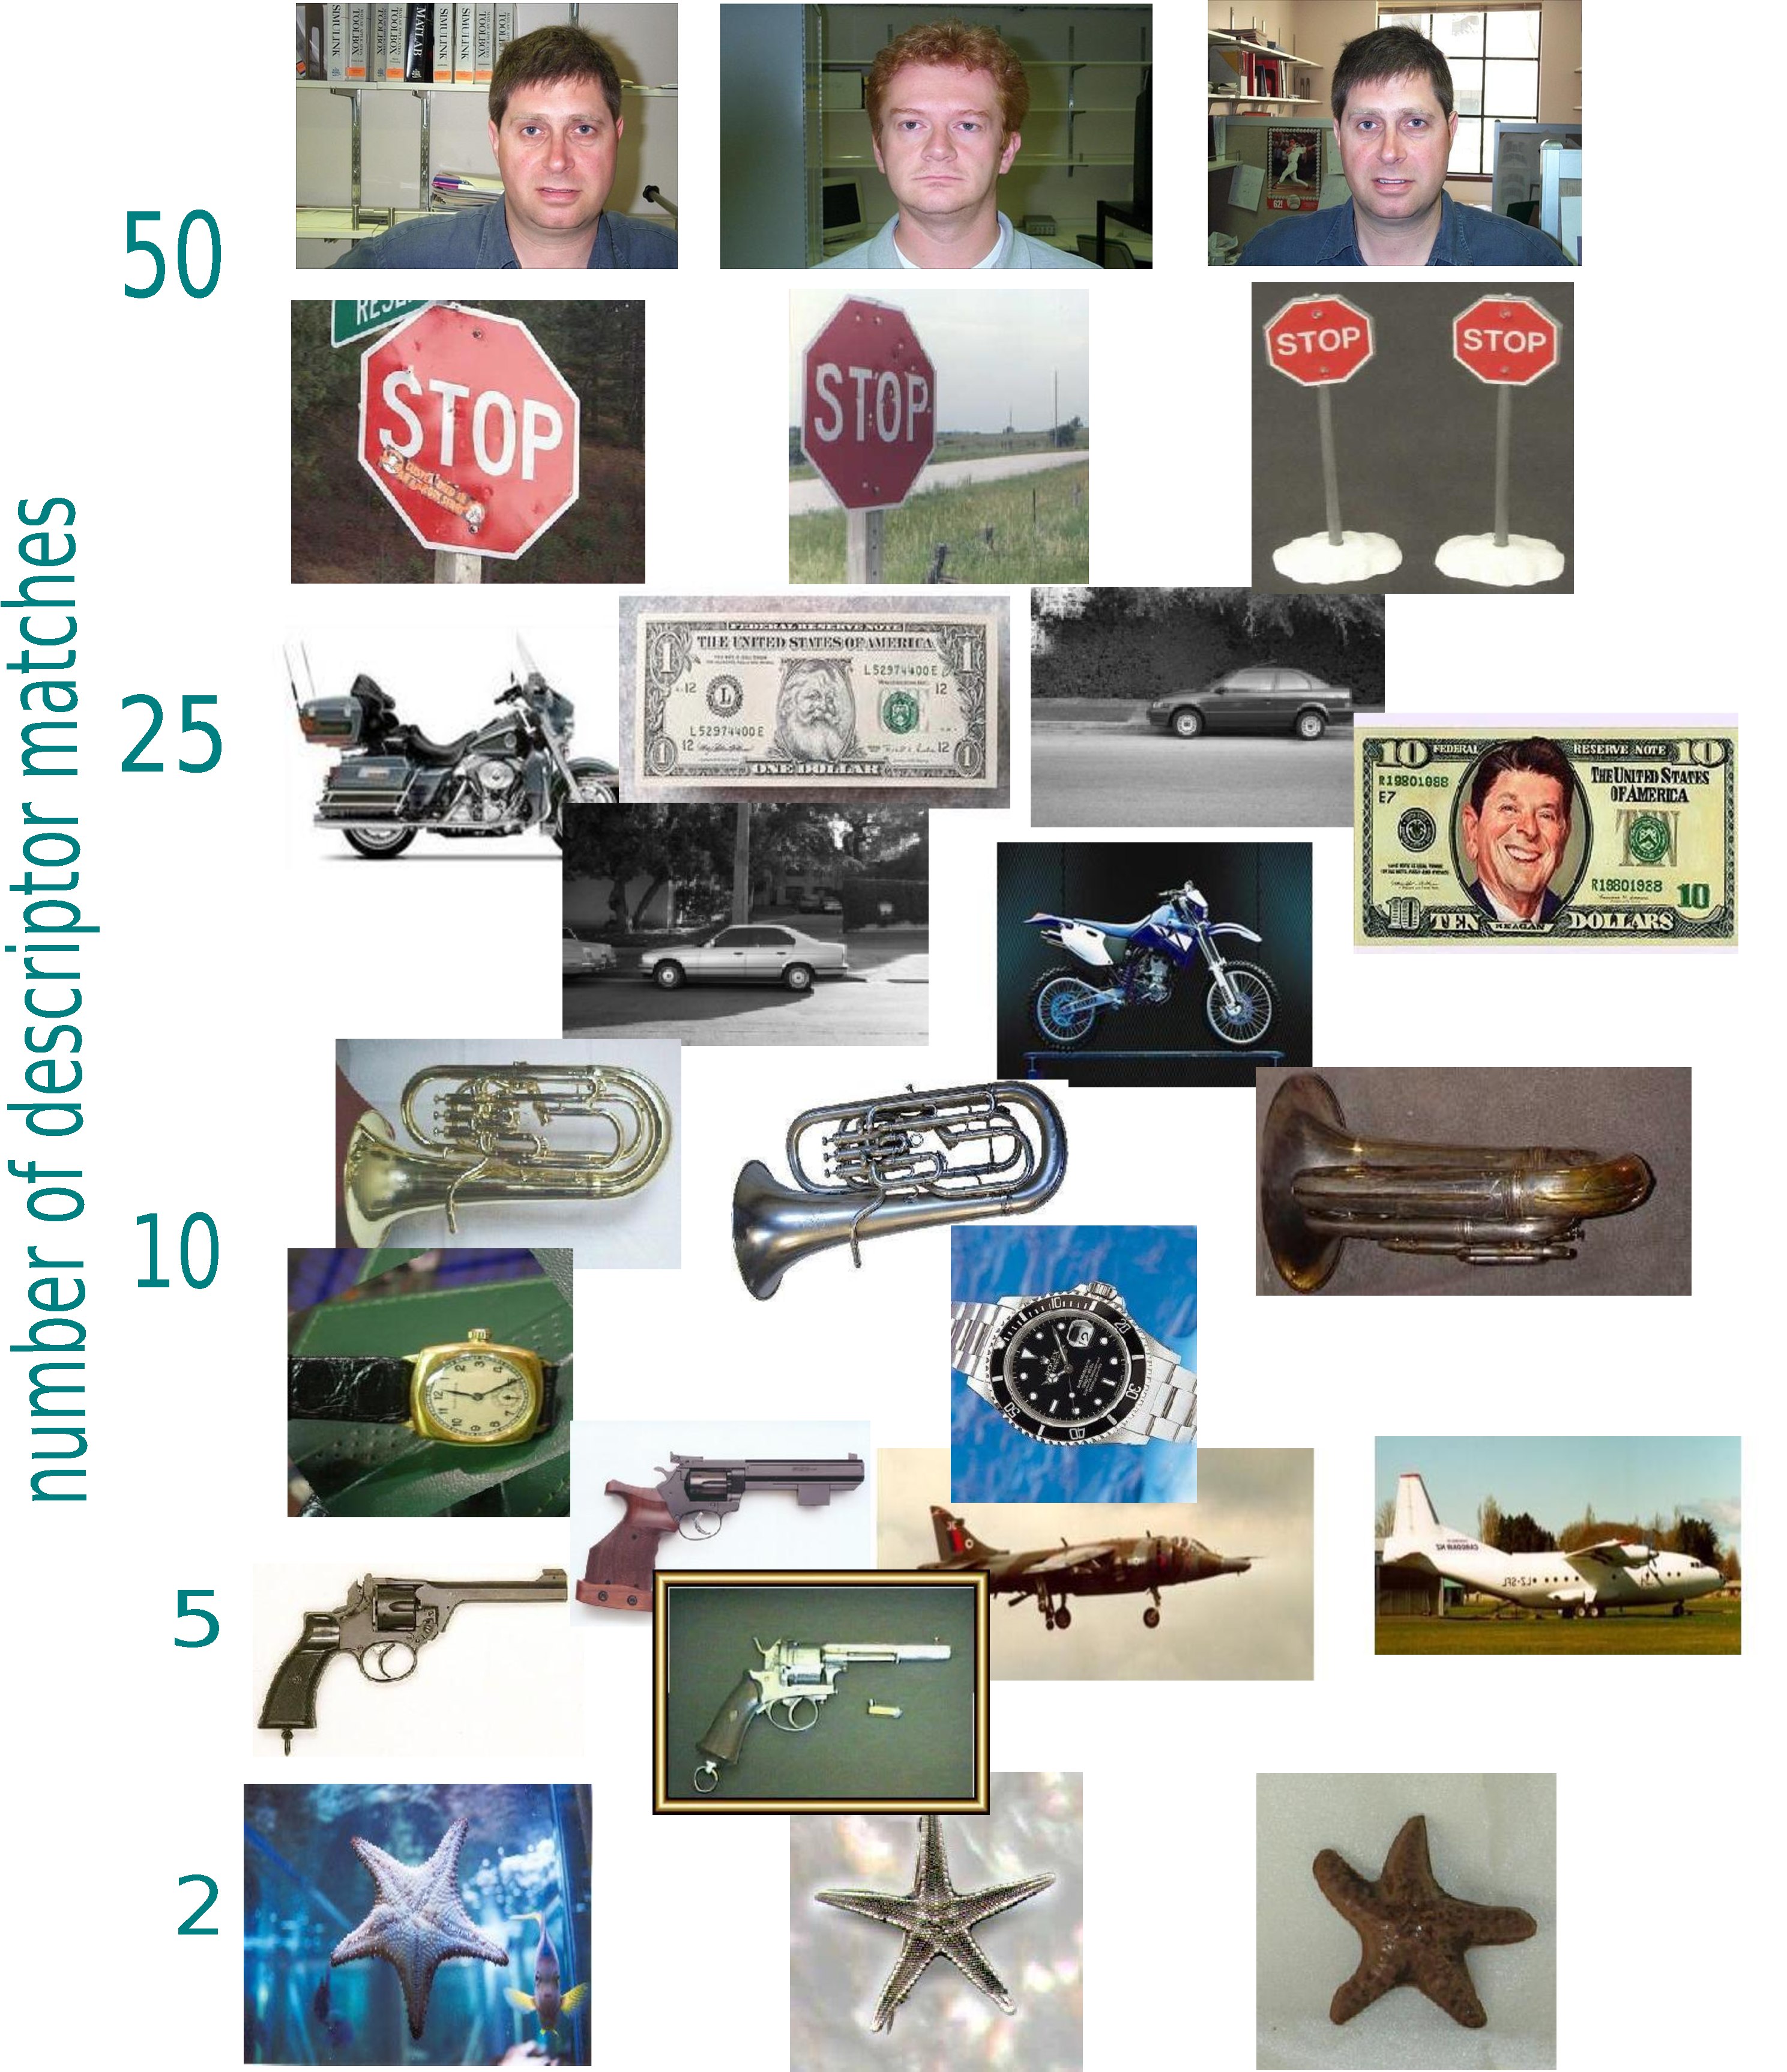
\includegraphics[width=0.8\linewidth]{resources/number_of_descriptor_matches.pdf}
  \caption{Typical amounts of descriptor matches between two random class examples.\label{fig:teaser}}
\end{center}
\end{figure}
%

Various methods have been proposed for detecting interest
points/regions and to construct descriptors from them,
most of which are designed with a different application in mind.
Recently, fast detectors and descriptors have been
proposed: SURF~\cite{BayEssTuy:2008},
FREAK~\cite{freak}, ORB~\cite{orb}, BRISK~\cite{brisk},
BRIEF~\cite{brief}. In~\cite{MikTuySch:2005} detectors
were evaluated by their repeatability ratios and total number of 
correspondences over several views of scenes and with various
imaging distortion types.
In~\cite{MikSch:2005}
descriptors were evaluated by their matching
rates for the same views. Comparisons on object classification
were
reported in \cite{ZhaMarLaz:2006} and
\cite{MikLeiSch:2005}, but they were tied to a single approach,
visual Bag-of-Words (BoW).
Our main contributions are:
\begin{compactitem}
\item We introduce intuitive detector and descriptor evaluation frameworks
by extending the detector and descriptor benchmarks
in~\cite{MikTuySch:2005,MikSch:2005} to intra-class
repeatibility and matching.
\item We evaluate the recent and popular detectors and descriptors and their various 
  implementations with the proposed framework.
\item We investigate the effect of using multiple best matches ($K=1,2,\ldots$) and
  introduce an alternative performance measure: {\em match coverage}.
\end{compactitem}
From the experimental results on Caltech and ImageNet classes we
arrive at the following important findings:
\begin{compactitem}
\item Dense SIFT features are the best.
\item Detectors generally perform well, but the ability of descriptors to match
  regions over visual class examples is poor (Fig.~\ref{fig:teaser}).
\item Using multiple---even a few---best matches instead of the single best
  provides significant improvement.
\item Dense grid sampling outperforms interest point detectors with a clear margin, but
\item object pose variation can drastically affect dense sampling
  while the best detector (Hessian-affine) is unaffected.
\item The original SIFT is still the best descriptor. % to all recent fast descriptors.
\end{compactitem}
Source code for the evaluation framework will be published in the
Web\footnote{\url{https://bitbucket.org/kamarain/descriptor_vocbenchmark}}. In addition, we verify our findings with the application of unsupervised
object class alignment where the best detector-descriptor pair
improves the state-of-the-art.

%
\subsection{Related work}
%
%\commentNK{I feel that this section is a bit thin. It depends a bit how aggressively we want to play it. Then the arguments should be better prepared.}


We believe that the general evaluation principles in~\cite{MikTuySch:2005,MikSch:2005} also hold in
the context of visual object classes: 1) \textit{detectors which return the same object regions for class
examples are good detectors} -- detection repeatability; 2)
\textit{descriptors which match the same object regions between class examples are good descriptors} -- match count/ratio. We refer to these repeating and matching regions as
``category-specific landmarks''. A qualitative measure to visualize
descriptors (``HOGgles'') was recently proposed by Vondrick et al.~\cite{VonKhoMal:2013},
but its main use is in visualization. More
quantitative evaluations were reported by Zhang et al.~\cite{ZhaMarLaz:2006}
and Mikolajczyk et al.~\cite{MikLeiSch:2005}, but these were
tied to a single methodology, the visual
Bag-of-Words (BoW)~\cite{SivZis:2003,CsuDanWil:2004}.
% Indeed, a successful outcome of the categorisation task is important
%for the final application, and therefore \cite{ZhaMarLaz:2006} compared different
%detectors and descriptors using a baseline BoW method. In the baseline method, codebooks are constructed from
%the raw descriptors and then images are categorised according to their codebook histograms.
%In their work, \cite{MikLeiSch:2005}
%were more specific by measuring average precision of feature clusters to represent a single class,
%entropy of spatial location distribution produced by a single cluster (ideally compact) and complementarity
%of different detectors. Both evaluations are biased by
%the selected BoW approach.
In this work, we show that the original evaluation principles can 
be adopted to obtain similar quantitative performance measures in general,
comparable and intuitive forms to the original works of Mikolajczyk et al., and not
tied to any specific approach.

% Note that IEEE typically puts floats only at the top, even when this
% results in a large percentage of a column being occupied by floats.


% An example of a double column floating figure using two subfigures.
% (The subfig.sty package must be loaded for this to work.)
% The subfigure \label commands are set within each subfloat command,
% and the \label for the overall figure must come after \caption.
% \hfil is used as a separator to get equal spacing.
% Watch out that the combined width of all the subfigures on a 
% line do not exceed the text width or a line break will occur.
%
%\begin{figure*}[!t]
%\centering
%\subfloat[Case I]{\includegraphics[width=2.5in]{box}%
%\label{fig_first_case}}
%\hfil
%\subfloat[Case II]{\includegraphics[width=2.5in]{box}%
%\label{fig_second_case}}
%\caption{Simulation results.}
%\label{fig_sim}
%\end{figure*}
%
% Note that often IEEE papers with subfigures do not employ subfigure
% captions (using the optional argument to \subfloat[]), but instead will
% reference/describe all of them (a), (b), etc., within the main caption.


% An example of a floating table. Note that, for IEEE style tables, the 
% \caption command should come BEFORE the table. Table text will default to
% \footnotesize as IEEE normally uses this smaller font for tables.
% The \label must come after \caption as always.
%
%\begin{table}[!t]
%% increase table row spacing, adjust to taste
%\renewcommand{\arraystretch}{1.3}
% if using array.sty, it might be a good idea to tweak the value of
% \extrarowheight as needed to properly center the text within the cells
%\caption{An Example of a Table}
%\label{table_example}
%\centering
%% Some packages, such as MDW tools, offer better commands for making tables
%% than the plain LaTeX2e tabular which is used here.
%\begin{tabular}{|c||c|}
%\hline
%One & Two\\
%\hline
%Three & Four\\
%\hline
%\end{tabular}
%\end{table}


% Note that IEEE does not put floats in the very first column - or typically
% anywhere on the first page for that matter. Also, in-text middle ("here")
% positioning is not used. Most IEEE journals use top floats exclusively.
% Note that, LaTeX2e, unlike IEEE journals, places footnotes above bottom
% floats. This can be corrected via the \fnbelowfloat command of the
% stfloats package.

%%%%%%%%%%%%%%%%%%

% An example of a floating figure using the graphicx package.
% Note that \label must occur AFTER (or within) \caption.
% For figures, \caption should occur after the \includegraphics.
% Note that IEEEtran v1.7 and later has special internal code that
% is designed to preserve the operation of \label within \caption
% even when the captionsoff option is in effect. However, because
% of issues like this, it may be the safest practice to put all your
% \label just after \caption rather than within \caption{}.
%
% Reminder: the "draftcls" or "draftclsnofoot", not "draft", class
% option should be used if it is desired that the figures are to be
% displayed while in draft mode.
%
%\begin{figure}[!t]
%\centering
%\includegraphics[width=2.5in]{myfigure}
% where an .eps filename suffix will be assumed under latex, 
% and a .pdf suffix will be assumed for pdflatex; or what has been declared
% via \DeclareGraphicsExtensions.
%\caption{Simulation Results}
%\label{fig_sim}
%\end{figure}

% Note that IEEE CS typically puts floats only at the top, even when this
% results in a large percentage of a column being occupied by floats.
% However, the Computer Society has been known to put floats at the bottom.


% An example of a double column floating figure using two subfigures.
% (The subfig.sty package must be loaded for this to work.)
% The subfigure \label commands are set within each subfloat command, the
% \label for the overall figure must come after \caption.
% \hfil must be used as a separator to get equal spacing.
% The subfigure.sty package works much the same way, except \subfigure is
% used instead of \subfloat.
%
%\begin{figure*}[!t]
%\centerline{\subfloat[Case I]\includegraphics[width=2.5in]{subfigcase1}%
%\label{fig_first_case}}
%\hfil
%\subfloat[Case II]{\includegraphics[width=2.5in]{subfigcase2}%
%\label{fig_second_case}}}
%\caption{Simulation results}
%\label{fig_sim}
%\end{figure*}
%
% Note that often IEEE CS papers with subfigures do not employ subfigure
% captions (using the optional argument to \subfloat), but instead will
% reference/describe all of them (a), (b), etc., within the main caption.


% An example of a floating table. Note that, for IEEE style tables, the 
% \caption command should come BEFORE the table. Table text will default to
% \footnotesize as IEEE normally uses this smaller font for tables.
% The \label must come after \caption as always.
%
%\begin{table}[!t]
%% increase table row spacing, adjust to taste
%\renewcommand{\arraystretch}{1.3}
% if using array.sty, it might be a good idea to tweak the value of
% \extrarowheight as needed to properly center the text within the cells
%\caption{An Example of a Table}
%\label{table_example}
%\centering
%% Some packages, such as MDW tools, offer better commands for making tables
%% than the plain LaTeX2e tabular which is used here.
%\begin{tabular}{|c||c|}
%\hline
%One & Two\\
%\hline
%Three & Four\\
%\hline
%\end{tabular}
%\end{table}


% Note that IEEE does not put floats in the very first column - or typically
% anywhere on the first page for that matter. Also, in-text middle ("here")
% positioning is not used. Most IEEE journals use top floats exclusively.
% However, Computer Society journals sometimes do use bottom floats - bear
% this in mind when choosing appropriate optional arguments for the
% figure/table environments.
% Note that, LaTeX2e, unlike IEEE journals, places footnotes above bottom
% floats. This can be corrected via the \fnbelowfloat command of the
% stfloats package.


%%%%%%%

%
\section{Comparing Detectors\label{sec:detectorcomparison}}
%
A good feature detector should detect local points or regions at the same
locations of class examples to make it possible to match corresponding ``parts''.
This criterion differs from~\cite{MikTuySch:2005}, where detectors were evaluated 
over views of same scenes corresponding to
specific object matching. In part-based object classification (e.g.,~\cite{FelGirMca:2010}),
%which has been adopted in the state-of-the-art approaches~\cite{FelGirMca:2010},
the descriptors (parts) should match despite substantial variance in their visual
appearance.
%Our case introduces a distinct and substantial
%source of variation: class visual appearance.\anders{I think this small motivation section
%may want to cite the part-based models (e.g. Feltzenwalb), since then we have an
%even stronger argument for saying that an object consists of distinct ``parts'',
%and that our new assumption is that feature descriptors should be able to match
%these parts over different instances of an object class.}

%
\subsection{Data\label{sec:data}}
%
%
\begin{figure}[h]
\begin{center}
  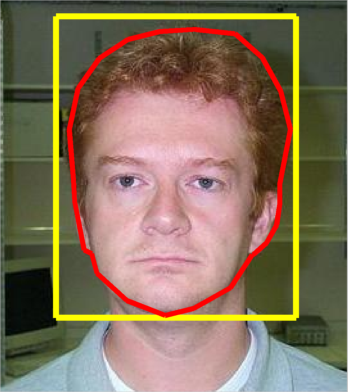
\includegraphics[width=0.25\linewidth]{resources/caltech-101_face_example.png}
  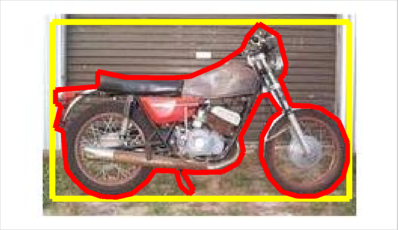
\includegraphics[width=0.4\linewidth]{resources/caltech-101_motorbikes_example.png}
  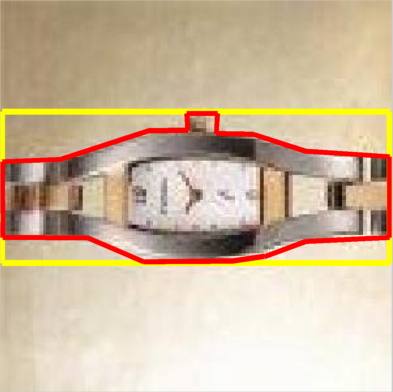
\includegraphics[width=0.25\linewidth]{resources/caltech-101_watch_example.png}\\
  \subfloat{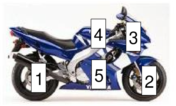
\includegraphics[height=0.18\linewidth]{resources/lm/lm_examples_cat02_img07.png}}
  \subfloat{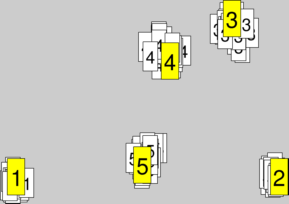
\includegraphics[height=0.18\linewidth]{resources/lm/lm_cat02.png}}
  \subfloat{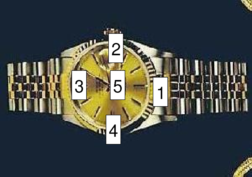
\includegraphics[height=0.15\linewidth]{resources/lm/lm_examples_cat10_img18.png}}
  \subfloat{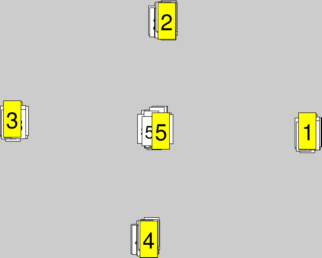
\includegraphics[height=0.15\linewidth]{resources/lm/lm_cat10.png}}
  \caption{Top: example images with the provided ground truth (bounding boxes and foreground regions).
    Bottom: landmark examples and multiple landmarks projected onto
    a single image (the yellow tags).
    \label{fig:caltech}}
  \end{center}
\end{figure}
%
The experiments were conducted with the Caltech-101~\cite{FeiFerPer:2006} images.
Caltech-101 is preferred as the baseline
%over the more recent data sets, such as
%Caltech-256~\cite{Caltech256}, Pascal VOC~\cite{EveGooWil:2010} and
%ImageNet~\cite{imagenet},
since objects' poses are roughly fixed that allows us to measure
the effect of appearance variation without geometric pose noise.
In the additional experiments we verify our results with randomly rotated
versions of the Caltech images and the recent
ImageNet database~\cite{imagenet}.
%they contain substantial 3D view point changes
%(e.g. car frontal vs. car side) which are not expected to be solved
%on the local feature level.
%For compactness and clarity, the results are reported for the following ten categories which
%represent well the overall performance variation: \textit{watch}, \textit{stop\_sign}, \textit{starfish},
%\textit{revolver}, \textit{euphonium}, \textit{dollar\_bill}, \textit{car\_side},
%\textit{airplanes}, \textit{Motorbikes} and \textit{Faces\_easy}.
The foreground masks were used to remove features detected
in the background (Fig.~\ref{fig:caltech}). Affine correspondence between category examples were established
by manually annotating 5-12 landmarks per category and estimating the pair-wise image
transformations using the direct linear transform~\cite{HarZis:2003} and linear interpolation.
%Examples with
%annotated landmarks are shown in Fig.~\ref{fig:affine_example1}.
25 random pairs from each class were repeatedly picked.
%% (tot. of 500 images).
%%
%\begin{figure}[h]
%\begin{center}
%\subfloat{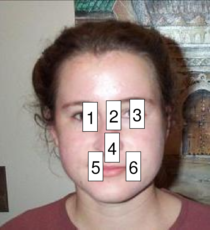
\includegraphics[height=0.2\linewidth]{resources/lm/lm_examples_cat01_img01.png}}
%\subfloat{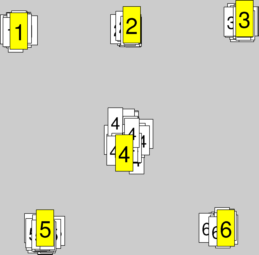
\includegraphics[height=0.2\linewidth]{resources/lm/lm_cat01.png}}~
%\subfloat{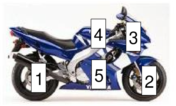
\includegraphics[height=0.2\linewidth]{resources/lm/lm_examples_cat02_img07.png}}
%\subfloat{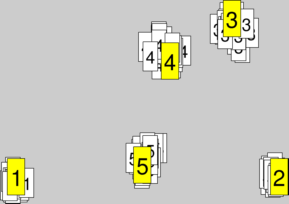
\includegraphics[height=0.2\linewidth]{resources/lm/lm_cat02.png}}\\
%%\subfloat{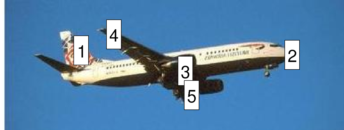
\includegraphics[height=0.1\linewidth]{resources/lm/lm_examples_cat03_img08.png}}
%%\subfloat{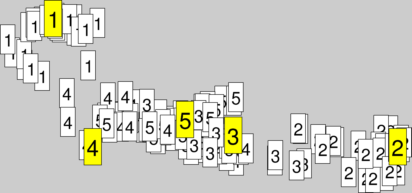
\includegraphics[height=0.1\linewidth]{resources/lm/lm_cat03.png}}~
%%\subfloat{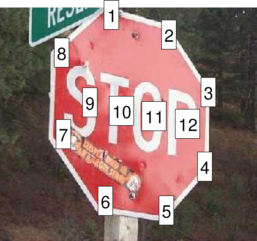
\includegraphics[height=0.16\linewidth]{resources/lm/lm_examples_cat09_img01.png}}
%%\subfloat{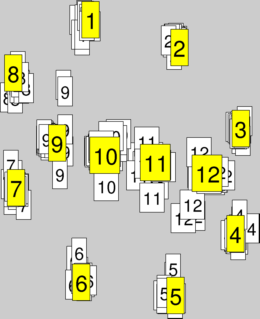
\includegraphics[height=0.16\linewidth]{resources/lm/lm_cat09.png}}\\
%%\subfloat{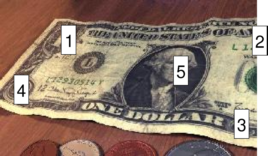
\includegraphics[height=0.12\linewidth]{resources/lm/lm_examples_cat05_img04.png}}
%%\subfloat{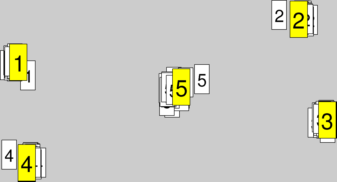
\includegraphics[height=0.12\linewidth]{resources/lm/lm_cat05.png}}~
%%\subfloat{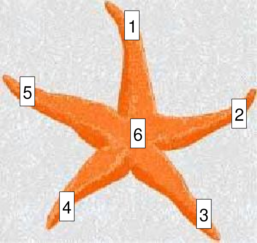
\includegraphics[height=0.14\linewidth]{resources/lm/lm_examples_cat08_img02.png}}
%%\subfloat{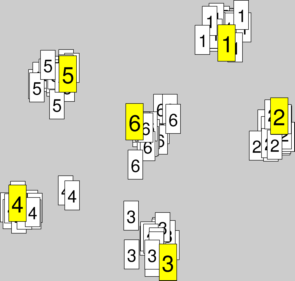
\includegraphics[height=0.14\linewidth]{resources/lm/lm_cat08.png}}\\
%%\subfloat{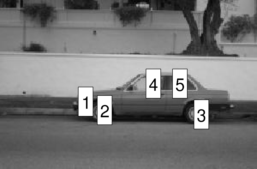
\includegraphics[height=0.14\linewidth]{resources/lm/lm_examples_cat04_img02.png}}
%%\subfloat{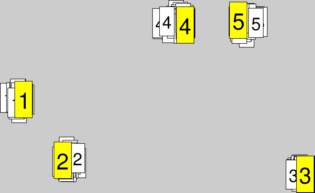
\includegraphics[height=0.14\linewidth]{resources/lm/lm_cat04.png}}~
%%\subfloat{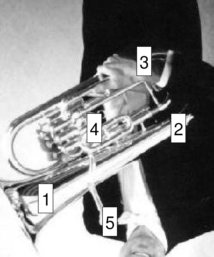
\includegraphics[height=0.14\linewidth]{resources/lm/lm_examples_cat06_img02.png}}
%%\subfloat{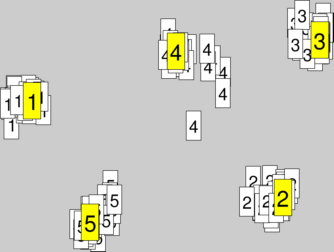
\includegraphics[height=0.14\linewidth]{resources/lm/lm_cat06.png}}\\
%\subfloat{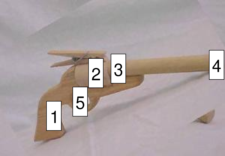
\includegraphics[height=0.17\linewidth]{resources/lm/lm_examples_cat07_img10.png}}
%\subfloat{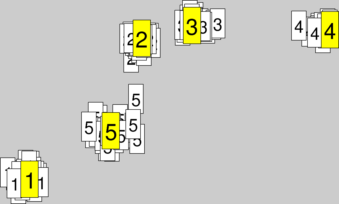
\includegraphics[height=0.17\linewidth]{resources/lm/lm_cat07.png}}~
%\subfloat{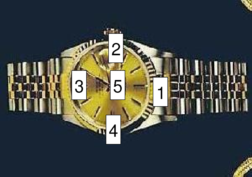
\includegraphics[height=0.17\linewidth]{resources/lm/lm_examples_cat10_img18.png}}
%\subfloat{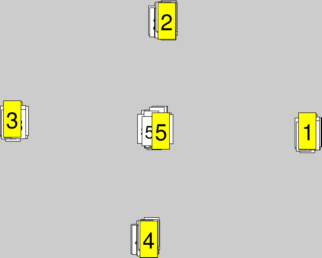
\includegraphics[height=0.17\linewidth]{resources/lm/lm_cat10.png}}
%\caption{Object class examples with annotated landmarks (leftmost in each image pair) and 50 examples (affine) projected into
%a single space (denoted by the yellow tags). The image diagonal normalised (resolution independent) two standard deviations are
%0.0158, 0.0297, 0.0486 and 0.0177, respectively. The part variances imply class specific spatial variance of object parts.}%  {\color{blue} Anders: does the last information on the landmarks tell something about the intra-class variation of the parts, or does this figure simply show the (small) spatial variation of the ``same''  parts for the four example classes?}}
% The two standard deviations of the image diagonal normalised projection errors are (from left to right and top to bottom):
%0.0158,
%0.0297,
%0.1701,
%0.0460,
%0.0304,
%0.0373,
%0.0194,
%0.0641,
%0.0486, and
%0.0177.
%\label{fig:affine_example1}
%\end{center}
%\end{figure}
%

%
\subsection{Feature detectors}
%
The detectors for the experiments were selected among the
best performing from our preliminary
study~\cite{LanKanKam:2012} and the recently proposed
detectors: BRIEF~\cite{brief}, BRISK~\cite{brisk}, ORB~\cite{orb} and
FREAK~\cite{freak}. The preliminary detectors were
\begin{compactenum}
\item Two implementations of the difference of Gaussian: \textit{sift} and \textit{dog-vireo}
\item Harris-Laplace: \textit{harlap-vireo}
\item Laplacian of Gaussian (log): \textit{log-vireo}
\item Three implementations of the Hessian-affine: \textit{hessaff}, \textit{hessaff-alt} and \textit{hesslap-vireo} 
\item Speeded-up robust features: \textit{surf}
\item Maximally stable extremal regions: \textit{mser}
\end{compactenum}
The detectors are publicly available:
 \textit{*-vireo} implementations in Zhao's
Lip-vireo toolkit (\url{http://code.google.com/p/lip-vireo}),
\textit{hessaff} and \textit{hessaff-alt} (by Mikolajczyk) at
\url{http://featurespace.org}, \textit{surf} at the
authors'~\cite{BayEssTuy:2008} web site and \textit{mser} and \textit{sift} in
the VLFeat toolbox (\url{http://vlfeat.org}). 
The best average repeatability was $33.7\%$ for \textit{dog-vireo} and the
best number of corresponding regions $57.4$ for \textit{hesslap-vireo}. The
best three detectors based on the both repeatability and number of regions were
\textit{hesslap-vireo} ($30.6\%$, $57.4$), \textit{hessaff} ($25.3\%$, $47.8$) and
log-vireo ($26.3\%$, $46.5$). We report results for the best:
the hessaff detector.
% and since detector-descriptor combinations using the hessaff
%detector were superior in our preliminary work, we selected hessaff for this
%work as well. In addition, to compare the ``original idea''
%by Lowe~\cite{Low:2004} and state-of-the-art, we also included SIFT detector
%from VLFeat toolbox.

The best result from the recent detectors was obtained with the ORB
OpenCV implementation (\url{http://opencv.org}) which is included
(\textit{orb}). Moreover,
dense sampling has replaced detectors in the top methods
(Pascal VOC 2011~\cite{VOC:2011}) and
we added the dense SIFT in VLFeat (\url{http://vlfeat.org})
to our evaluation (\textit{dense}).


%
\subsection{Performance measures and evaluation}
%
For the detector performance evaluation, we adopted the procedure in~\cite{MikTuySch:2005}
with the exception that
interest points detected outside the object area (Fig.~\ref{fig:caltech})
are removed.
%
For each image pair, points from the first image are projected onto the
second image by the
affine transformation estimated using the annotated landmarks.
%The landmarks projected on a randomly selected example of each category
%are demonstrated in Fig.~\ref{fig:affine_example1} with the
%two standard deviations corresponding to the 95\% error distributions.
%%Only features covered by
%%both images are considered, though in this case practically all the features
%%fulfill that requirement.
The interest points (regions) are described by 2D ellipses and when a transformed
ellipse overlaps with an ellipse in the second image a correct correspondence
is recorded.
%We thus have a {\em corresponding region}, or simply a {\em correspondence}.
The number and rate of correspondences for each detector is of interest. A detector performs well
if the total number is large and has high precision if the ratio of correct matches is high.
We used the parameter settings
from~\cite{MikTuySch:2005}: 60\% overlap threshold and normalization of the ellipses to
the radius of 30 pixels. The normalization is required since the overlap area depends
on the size of the ellipses. %\commentNK{This is a bit unclear for me but experts might now}

The reported performance numbers are the average number of correspences between
image pairs and the repeatability rate, i.e. the number of correspondences divided
by the total number of points.

\subsection{Results}
%
\begin{figure}[h]
\begin{center}
\subfloat[]{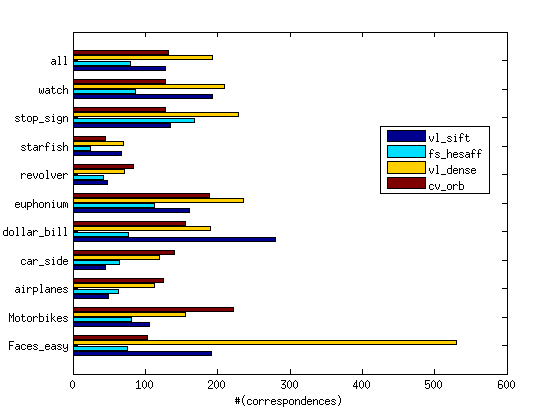
\includegraphics[width=0.9\linewidth]{resources/antti_results/ComparingDetectors/correspondences_metaPar.png}}\\
\subfloat[]{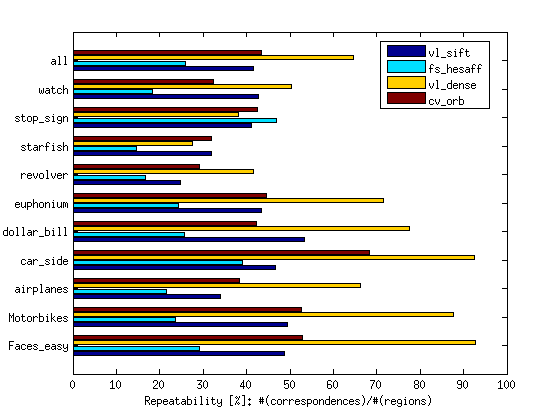
\includegraphics[width=0.9\linewidth]{resources/antti_results/ComparingDetectors/repRate_metaPar.png}}\\
%\subfloat[]{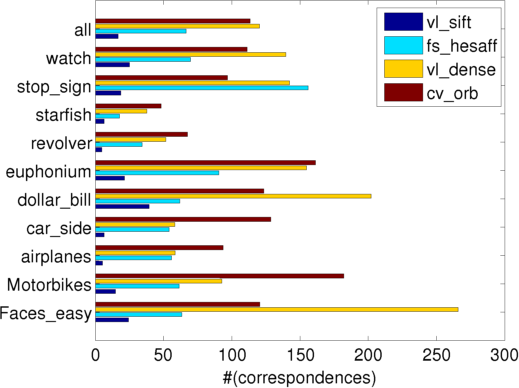
\includegraphics[width=0.8\linewidth]{resources/joni_results/PLOT_detectors_benchmark1report1-detcor-avg.png}}\\
%\subfloat[]{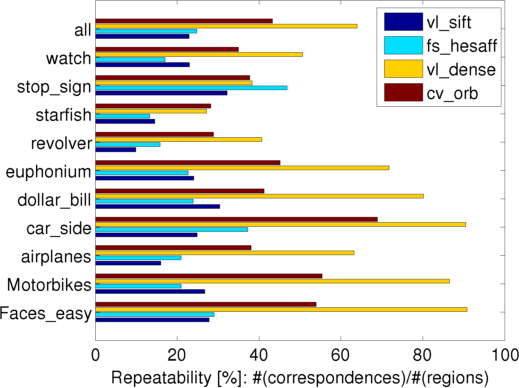
\includegraphics[width=0.8\linewidth]{resources/joni_results/PLOT_detectors_benchmark1report1-detrep-avg.png}}\\
%\subfloat[]{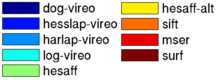
\includegraphics[width=0.3\linewidth]{resources/ville_results/detector-legend.png}}
\subfloat[]{\scriptsize
\begin{tabular}{l r r}
\toprule
\textit{Detector} & \textit{Avg \# of corr.} & \textit{Avg. rep. rate}\\
\midrule
%\textit{dog-vireo}     & 16.0 & 33.7\%\\
%\textit{hesslap-vireo} & 57.4 & 30.6\%\\
%\textit{harlap-vireo}  & 34.2 & 20.3\%\\
%\textit{log-vireo}     & 46.5 & 26.3\%\\
%\textit{hesaff}        & 47.8 & 25.3\%\\
%\textit{hesaff-alt}    & 25.0 & 23.4\%\\
%\textit{sift}          & 16.2 & 21.5\%\\
%\textit{mser}          & 11.7 & 13.8\%\\
%\textit{surf}          & 27.9 & 32.0\%\\
%{vl\_sift}       &  16.7 & 22.9\%\\
%{fs\_hessaff}    &  66.5 & 24.8\%\\
%{cv\_orb}        & 113.4 & 43.3\%\\
%{vl\_dense}       & 120.4 & 64.0\%\\
{vl\_sift}       &  127.5 & 41.6\%\\
{fs\_hessaff}    &  79.3 & 26.0\%\\
{cv\_orb}        & 132.0 & 43.5\%\\
{vl\_dense}       & 192.3 & 64.6\%\\
\bottomrule
\end{tabular}}
\caption{Detector evaluation in object class matching. Meta-parameters were set to return
on average 300 regions.
(a) average number of corresponding regions,
%\textit{dog-vireo}: 16.0;
%\textit{hesslap-vireo}: 57.4;
%\textit{harlap-vireo}: 34.2;
%\textit{log-vireo}: 46.5;
%\textit{hesaff}: 47.8;
%\textit{hesaff-alt}: 25.0;
%\textit{sift}: 16.2;
%\textit{mser}: 11.7;
%\textit{surf}: 27.9;
(b) repeatability rates,
%\textit{dog-vireo}: 33.7\%;
%\textit{hesslap-vireo}: 30.6\%;
%\textit{harlap-vireo}: 20.3\%;
%\textit{log-vireo}: 26.3\%;
%\textit{hesaff}: 25.3\%;
%\textit{hesaff-alt}: 23.4\%;
%\textit{sift}: 21.5\%;
%\textit{mser}: 13.8\%;
%\textit{surf}: 32.0\%;
%(c) colour coding of the detectors, and (d) overall results table.\label{fig:results1}}
and (c) the overall results table.\label{fig:results1}}
\end{center}
\end{figure}
%\begin{figure}[h]
%\begin{center}
%\subfloat[]{\includegraphics[width=0.9\linewidth]{resources/detcor-median.png}}
%\subfloat[]{\includegraphics[width=0.9\linewidth]{resources/detrep-median.png}}
%\caption{(a) median number of corresponding regions, (b) median repeatability rate.\label{fig:results1_median}}
%\end{center}
%\end{figure}
%
It is noteworthy that this experiment differs from our preliminary work
in the sense that instead of using the default parameters for each detector
we adjusted their meta-parameters to return on average 300 regions for
each image (see Sec.~\ref{sec:more_regions} for further analysis).
The results of the detector experiment  are shown in Fig.~\ref{fig:results1}.
%The main difference as compared to our preliminary work~\cite{LanKanKam:2012}
With the adjusted meta-parameters the difference between the detectors
is less significant than in our preliminary work~\cite{LanKanKam:2012} and
the previous winner, Hessian-affine, is now the weakest. The dense sampling
is clearly better than others, but otherwise the ORB detector seems
attempting due to its speed. It is also noteworthy that without the parameter
adjustment the results of the original SIFT detector would be by order of
magnitude worse.
Some less favorable
properties of dense sampling are discussed in Sec.~\ref{sec:challenging}.
%\anders{Should we note that the dense matching only performs so well (extremely high repeatability rates), simply because there is a small affine transformation between the 25 sampled image pairs in each category? Otherwise, the reader may think we've found a holy grail. The dense sampling would e.g. not perform so well for Mikolajczyk's benchmark, right?}
%There are significant differences between the different categories.
%Dollar bill and stop sign are generally the easiest, as expected due to
%lower variation in their visual appearance, while the airplanes, car side views and revolvers are
%the most difficult. For the airplanes this
%can be explained by the fact that one of the landmarks is placed on the wing resulting in
%3D pose changes instead of 2D affinities.
%The numbers for all categories are by order of magnitude smaller than for the fixed
%scenes in~\cite{MikTuySch:2005}, being tens of correspondences instead of hundreds of
%them.
%\commentNK{What do we learn from that? Categorization is quite a different problem requiring probably features with higher level of abstraction}

\subsection{Detecting more regions\label{sec:more_regions}}
%
\begin{figure}[h]
  \begin{center}
    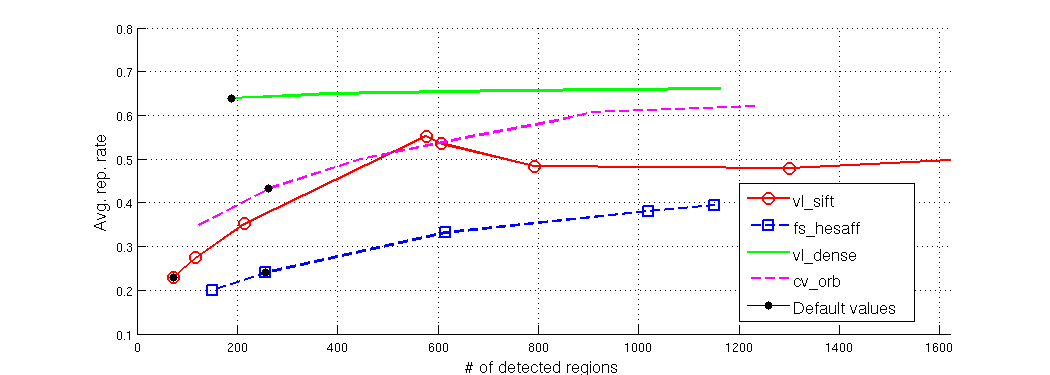
\includegraphics[trim=60 0 40 0, clip=true, width=0.99\linewidth]{resources/antti_results/DetectingMoreRegions/DetectorPlot.png}
    \caption{Detector repeatability as the function of the number of
      detected regions adjusted by the meta-parameters (defaults
      marked by black dots).\label{fig:more_regions}}
  \end{center}
\end{figure}
%
In the previous example, we adjusted detector meta-parameters to
return on average 300 regions for each image. That made detectors
produce very similar results while using the default parameters in
our previous work lead to completely different interpretation. 
It is interesting to study whether we can exploit meta-parameters
further to increase the number of corresponding regions.
For ORB we adjusted the edge threshold, for
Hessian-affine the feature density and the Hessian threshold,
for SIFT the number of levels per octave, and for the dense
the grid step size.
%dense sampling, but in the next descriptor evaluation it turns out that
%more regions or better descriptors are needed. Therefore we briefly study
%the problem of having more regions with the best performing methods.
%This is achieved by changing the meta-parameters for the detectors
%ORB, the Hessian-affine, the dense sampling and SIFT. Using the OpenCV
%implementation of ORB we modified the {\em edgeThreshold}-parameter
%which affects the size of the border where the features are detected.
%For the Hessian-affine we changed the feature density per pixels ({\em
%density}) and the {\em hessian threshold} -parameter. With the dense
%sampling we modified step size ({\em step}) and for SIFT we adjusted
%the number of levels per octave of the DoG scale ({\em Levels}) to get more regions.
%\joni{Antti: kuvaa tassa mitka nama parametrit ovat seuraaville: sift, hessaff, orb, dense ja lisaa kuvaaja (eli repeatability rate vs. average number of extracted regions - tsekkaa myos SIFT:in ihme dipin syy}
We computed the detector repeatability rates as the functions of the
number of detected regions (see Figure~\ref{fig:more_regions}). As
expected the meta-parameters have almost no effect to the dense detection
while Hessian-affine, ORB and especially SIFT clearly improve as the
number of regions increase (SIFT regions saturate to the same
locations approx. at 600 detected regions). For the most difficult
classes in Fig.~\ref{fig:results1} (starfish and revolver) more
regions is beneficial opening a novel
research direction whether the detector parameters should be
optimized for class detection?


%------------------------------------------------------------------------- 
%
\section{Comparing Descriptors\label{sec:descriptorcomparison}}
%
A good region descriptor for object matching should be
discriminative to match only correct regions, and also tolerate
small appearance variation between the examples.
The descriptor performances were obtained in the original
work~\cite{MikSch:2005} by computing statistics of the correct and false
matches. Between different class examples, descriptor matches are expected to
be weaker due to increased appearance variation.
For example, scooters and road bikes are both in the
Caltech-101 motorbikes category, but their pair-wise similarity
is much weaker than between two scooters or two road bikes.
%Moreover, there is natural variation in the spatial configurations
%of the regions (constellation deformation).
%Therefore, we
%need to tailor the original method to cope with these two sources
%of variation.

%It turns out that there is a strong discrepancy between mean and median
%results and therefore we propose an alternative measure, {\em coverage}, which
%measures the number of images ``covered'' with at least the given number $N$ of correspondences (coverage-$N$). 
%This complements the original evaluation criteria, since we get
%quantitative numbers for how many image pairs at least $N$ 
%correct matches can be found - a few pairs of huge number of matches
%do not distort the results as with the mean number of matches.


%To evaluate the performance of local descriptors selected we simply
%count matches and calculate statistics out of them. Test protocol used in
%\cite{MikSch:2005} is not suitable for this evaluation because the task for
%descriptors is not exactly the same. As we are searching for matches between
%various items in the same object category, the number of matches we can
%assume to be found is significantly lower than if we would try to find
%matches between two images taken at the same scene.

%Although the task of finding matches is not easy, in many cases several 
%matches can be found. If a few matches for an image pair is enough, depends on
%the application. Combining matches of several methods is also a possibility
%that can increase the number of found matches especially when there are
%different kinds of source images in use.

%We use term ``coverage'' to show in how many of the image pairs descriptor
%matches were found. Coverage-n then shows the pairs where $ n $ or more
%matches are found. It can reveal some properties of descriptors as some
%have ability to obtain a few matches even in very challenging image pairs 
%that with most descriptors no matches can be found. It is important to note that
%used detector affects this as it determines the spatial locations in the 
%image that descriptors are calculated for.

%
\subsection{Available descriptors}
%
This experiment is conducted using detector-descriptor
pairs. Our preliminary set of descriptors was:
\begin{compactenum}
\item Hessian-affine and SIFT
\item Hessian-affine and steerable filters
\item Vireo implementation of Hessian-affine and SIFT
\item Original SIFT detector and SIFT descriptor
\item Alternative (Vireo) implementation of SIFT and SIFT
\item SURF and SURF
\end{compactenum}
With their default parameters the combinations 1) and 2) utilizing
Mikolajczyk's implementation of Hessian-affine detector were
clearly superior to other methods~\cite{LanKanKam:2012}, but here
we adjust the meta-parameters to
return the same average number of regions (300).
%The Hessian-affine and SIFT achieved the average number of matches
%$66.1$ and median $46.0$.

To these experiments, we also include the best fast detector-descriptor
pair: ORB and BRIEF.
The following combinations will be reported:
{\em vl\_sift+vl\_sift} (FeatureSpace implementation),
{\em fs\_hessaff+fs\_sift} (FeatureSpace implementation),
{\em cv\_orb+cv\_brief} (OpenCV implementation),
{\em cv\_orb+cv\_sift} (OpenCV, to compare SIFT and BRIEF),
{\em vl\_dense+vl\_sift} (VLFeat implementation).
%
We also tested the RootSIFT descriptor
from~\cite{AraZis:2012} that achieved better performance in
their experiments, but in our case it
provided insignificant difference to the original SIFT
(mean: $3.9 \rightarrow 4.2$, median: $1 \rightarrow 1$). 

%
\subsection{Performance measures and evaluation\label{sec:descrperformance}}
In our preliminary work~\cite{LanKanKam:2012} we used a simplified
version of the Mikolajczyk's descriptor performance measure: the ellipse
overlap was replaced by normalized centroid distance of the matching
regions. However, the results by the simplified rule turned out to be
too optimistic and in this work we adopt the original measure. The
rule is the same as with the detectors, if the best matching regions
have sufficient overlap the match is counted correct.
Descriptors are computed for
all detected regions (foreground only). Images are processed
pair-wise and the best match for each region is selected from
the full distance matrix.
It is worth noting
that the rule proposed in~\cite{Low:2004} for discarding ``bad regions''
(ratio between the first and the second best is less than $1.5$) is
not used since it results complete failure.
We used the ellipse
overlap threshold $50\%$ from~\cite{MikSch:2005}, but also more strict
thresholds were tested.
Our performance numbers are the average number of matches and median
number of matches. In the detector evaluation the mean and median
numbers were almost the same, but here we report the both since
for the descriptors there is significant discrepancies between the mean
and median numbers.
%The median is used to suppress the effect of
%several too well matching pairs (same person, identical
%stop signs, etc.)
%
%For applications, it is also important to know how many matches
%are guaranteed to be found, and thus,
%%This can vary between images and is not uniform if the difference between the
%%average and median is large. Thus,
%we also report ``coverage'' numbers (Sec.~\.
%%, i.e. a 
%%number of image pairs for which at least N matches have been found
%%({\em coverage-N}). \anders{I don't think we need to re-explain the coverage term here, so we could remove the ``, i.e...'' part from this sentence.}

%
\subsection{Results\label{sec:results1}}
%
%
\begin{figure}[h]
\begin{center}
\subfloat[]{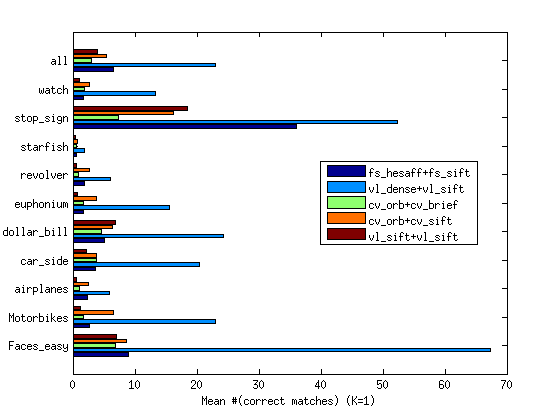
\includegraphics[width=0.9\linewidth]{resources/antti_results/DescriptorResults/numOfAvgMatchMean.png}}\\
%\subfloat[]{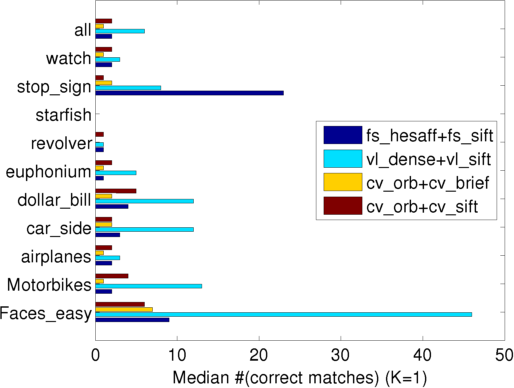
\includegraphics[width=0.8\linewidth]{resources/joni_results/result-figure-report1-median-all-besmatches-1.png}}\\
\subfloat[]{%
{\small
\begin{tabular}{l r r r r}
\toprule
\textit{Detector+descriptor} & \textit{Avg \#} & \textit{Med \#} & \textit{Avg \# (60\%)} & \textit{(70\%)}\\
\midrule
{vl\_sift+vl\_sift}         &  3.9 & 1 & 2.8 & 1.6 \\
{fs\_hessaff+fs\_sift}      &  6.5 & 2 & 5.9 & 4.9 \\
{vl\_dense+vl\_sift}        & 23.0 & 10 & 22.3 & 20.2 \\
{cv\_orb+cv\_brief}         &  3.0 & 1 & 2.9 & 2.7 \\
{cv\_orb+cv\_sift}          &  5.4 & 2 & 4.8  & 4.1 \\
\bottomrule
\end{tabular}}
} % End subfloat
\caption{Descriptor evaluation: (a) average number of matches per class,
%\textit{sift+sift}: 2.6;
%\textit{hesaff+gloh}: 6.3;
%\textit{surf+surf}: 2.75;
%\textit{hessaff+sift}: 6.3;
%\textit{dog-vireo+sift-vireo}: 2.6;
%\textit{hesslap-vireo+sift-vireo}: 3.4;
%(b) median,
%\textit{sift+sift}: 1.0;
%\textit{hesaff+gloh}: 0.0;
%\textit{surf+surf}: 1.0;
%\textit{hessaff+sift}: 0.0;
%\textit{dog-vireo+sift-vireo}: 1.0;
%\textit{hesslap-vireo+sift-vireo}: 0.5;
%(c) colour coding of the method names, and
(b) overall results table. The default overlap threshold is 50\%~\cite{MikSch:2005}, 
60\% and 70\% results demonstrate the effect of the more strict overlaps.}
\label{fig:results2}
\end{center}
\end{figure}
%
%The data for this experiment were the same.
The average and median number of matches for the descriptor evaluation
are shown in Fig.~\ref{fig:results2}.
For many classes, the mean and median numbers are very low and
dense grid sampling is superior for
all classes, achieving the average of $23.0$ and median of $10.0$ matches.
The more strict overlaps, $60\%$ and $70\%$, provide almost the same numbers
verifying that the matched regions do match well also spatially.
%The
%result is verified by the coverage results in Fig.~\ref{fig:results3}
%where the dense sampling based SIFT finds at least 6 matches
%from 13 our 25 images on average. The next best is the Hessian-affine
%with 7 out of 25.
%The only exception is the stop signs category for
%which the Hessian-affine outperforms dense sampling.

The best results were obtained for the stop signs, dollar bills and
faces, but the overall performance is poor.
The best discriminative methods could still learn to detect these
categories, but it is difficult to imagine naturally emerging
``common codes'' for other classes except the three.
It is surprising that the best detectors, Hessian-affine and dense
sampling, were able to provide $79$ and $192$, repeatable regions
on average, but only roughly $10\%$ of these match in the descriptor space.
Despite the fact that the SIFT detector performed well in the detector
experiment, its regions do not match well in this experiment.
The main conclusion of these results is that all descriptors perform
poorly in matching regions between class examples.

\subsection{The more the merrier?\label{sec:more_matches}}
Similar to Sec.~\ref{sec:more_regions} we study how the average number
of matches behaves as the function of the number of extracted regions.
This is justified as some works claim that
``the more the merrier''~\cite{NowJurTri:2006}. The result graph is shown in
Figure~\ref{fig:more_matches}. The results show that adding more regions
by adjusting the detector meta-parameters provides only minor
improvement to the average number of matches. Clearly, the ``best regions''
are provided first and dense sampling performs much better indicating
that what is ``interesting'' for the detectors is not necessarily a good
object part.
\begin{figure}[h]
  \begin{center}
    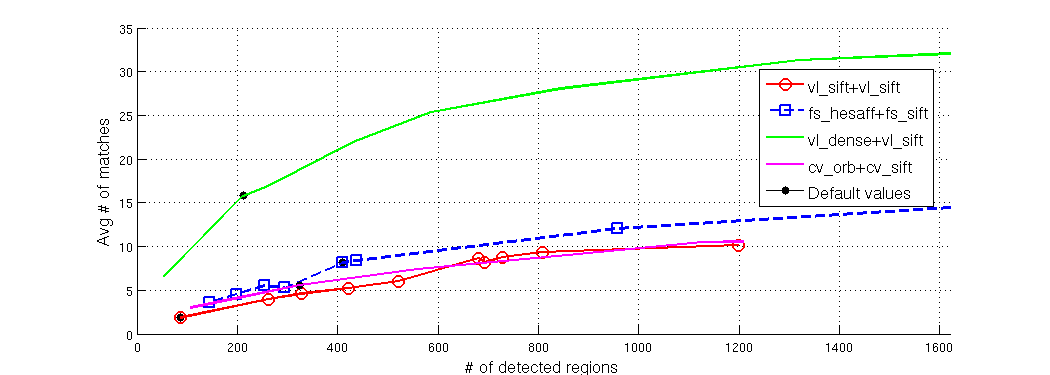
\includegraphics[trim=60 0 40 0, clip=true, width=0.99\linewidth]{resources/antti_results/DetectingMoreRegions/DescriptorPlot.png}
    \caption{Descriptors' matches as functions of the number
      of detected regions controlled by the meta-parameters (default values denoted by black dots).
      \label{fig:more_matches}}
  \end{center}
\end{figure}


%%%%%%%%%%%%%%%%%%%%%%%%%
\section{Advanced analysis}
%
In this section, we address the open questions raised during the
detector and descriptors comparisons in Section~\ref{sec:detectorcomparison}
and~\ref{sec:descriptorcomparison}. The important
questions are: why only a few matches are found between different class
examples and what can be done to improve that? Why dense sampling outperforms
all interest point detectors and does it have any drawbacks? Do our results
generalize to other datasets?

%
\subsection{ImageNet classes}
%
To validate our results, we selected 10 different categories from the
the state-of-the-art object detection database: ImageNet~\cite{imagenet}.
The images were scaled to the same size as the Caltech-101 images and
the foreground areas were annotated. The results for the ImageNet classes
are in Figure~\ref{fig:results2_imagenet}. The average number of matches
is roughly half of the number of matches with Caltech-101 images which
can be explained by the fact that the dataset is more challenging
due to 3D view point changes. However, the ranking of
the methods is almost the same: dense sampling and
SIFT is the best and SIFT detector and descriptor pair is the
worst. The results validate our findings with Caltech-101.
%
\begin{figure}[h]
\begin{center}
\subfloat[]{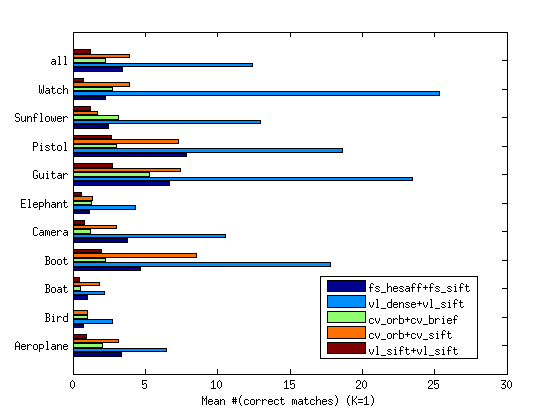
\includegraphics[width=0.9\linewidth]{resources/antti_results/Imagenet_results/mean.png}}\\
%\subfloat[]{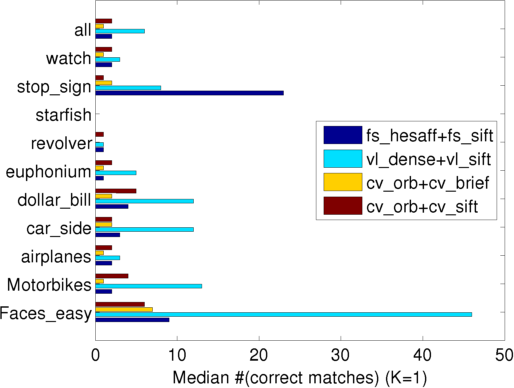
\includegraphics[width=0.8\linewidth]{resources/joni_results/result-figure-report1-median-all-besmatches-1.png}}\\
\subfloat[]{%
{\small
\begin{tabular}{l r r r r}
\toprule
\textit{Detector+descriptor} & \textit{Avg \#} & \textit{Med \#} & \textit{Avg \# (60\%)} & \textit{(70\%)}\\
\midrule
{vl\_sift+vl\_sift}         &  1.2 & 0 & 0.7 & 0.3 \\
{fs\_hessaff+fs\_sift}      &  3.4 & 2 & 2.8 & 1.9 \\
{vl\_dense+vl\_sift}        & 12.4 & 7 & 11.6 & 10.2 \\
{cv\_orb+cv\_brief}         &  2.2 & 1 & 1.9 & 1.5 \\
{cv\_orb+cv\_sift}          &  3.9 & 2 & 3.3 & 2.5 \\
\bottomrule
\end{tabular}}
} % End subfloat
\caption{Descriptor evaluation with the ImageNet classes to
verify results in Fig.~\ref{fig:results2}.\label{fig:results2_imagenet}}
\end{center}
\end{figure}



%
\subsection{Beyond the single best match}
%
%It is obvious that descriptors match better between two images of a same
%scene than two different examples of a same object class. However,
%it can be assumed that on average two descriptors describing
%the same object part should match better than two distant parts.
%To test this assumption, every descriptor
%can be assigned to multiple best matches.
In object matching, assigning each descriptor to several best matches,
``soft assignment''~\cite{AgaTri:2008,TuySch:2007,ChaLemVed:2011},
provides improvement and we want to experimentally verify this
finding using our framework. To measure the effect of multiple assignments, we
establish a new performance measure: \textit{coverage}. Coverage
corresponds to the number of image pairs for which at least N matches
have been found ({\em coverage-N}) and this measure is more meaningful
than the average number of matches since there was strong discrepancies
between the average and median numbers.
We tested the multiple assignment procedure by accumulating matches over
$n = 1, 2, \ldots, K$ best matches. The corresponding coverage for
$K = 1, 5, 10$ are shown in Fig.~\ref{fig:coverage}. Obviously,
more image pairs contain at least $N=5$ than $N=10$ matches.
With $K=1$ (only the best match) the best method, VLFeat dense SIFT,
finds at least $N=5$ matches in 16 out of
25 image pairs and 13 for $N=10$. When the number of best
matches is increased to $K=5$, the same numbers are 19 and 18, respectively,
showing clear improvement. Beyond $K=5$ the positive effect diminishes and
also the difference between the methods is less significant.
%, but
%it is clearly beneficial to use more than one best match of each
%region.
%
\begin{figure*}[htbp]
\begin{center}
\subfloat{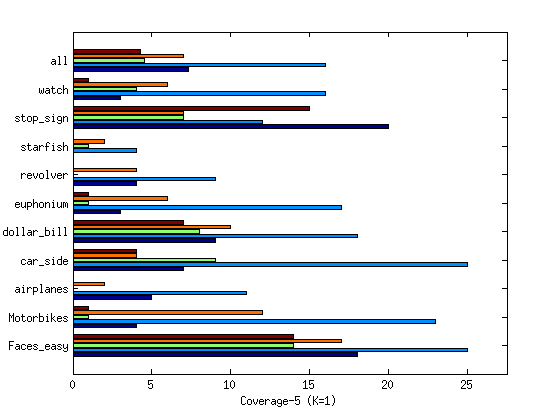
\includegraphics[height=0.28\linewidth]{resources/antti_results/BeyondSingleBestmatch/metaPar_Cov5_K1.png}}
\subfloat{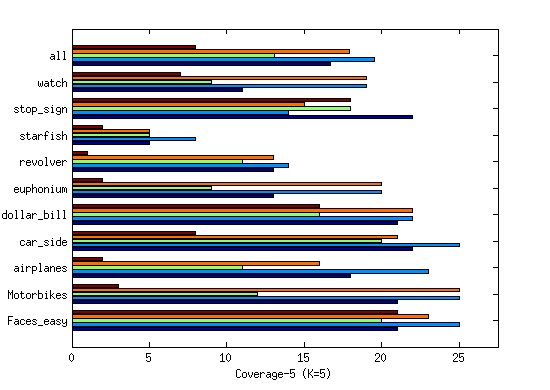
\includegraphics[trim=55 0 0 0, clip=true, height=0.28\linewidth]{resources/antti_results/BeyondSingleBestmatch/metaPar_Cov5_K5.png}}
\subfloat{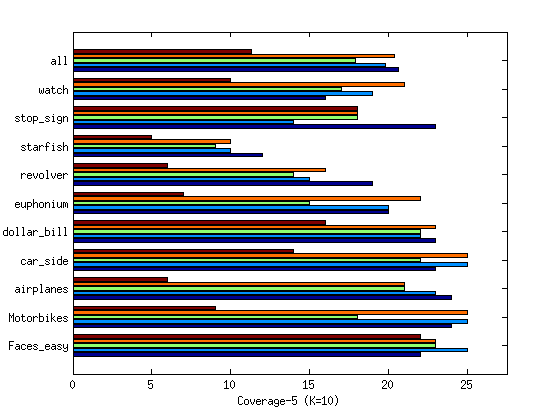
\includegraphics[trim=55 0 0 0, clip=true, height=0.28\linewidth]{resources/antti_results/BeyondSingleBestmatch/metaPar_Cov5_K10.png}}

\subfloat{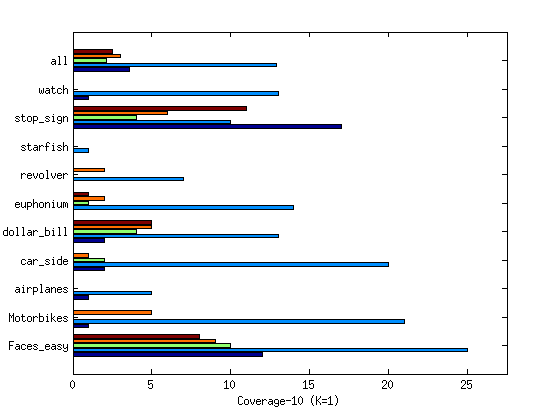
\includegraphics[height=0.28\linewidth]{resources/antti_results/BeyondSingleBestmatch/metaPar_Cov10_K1.png}}
\subfloat{\includegraphics[trim=75 0 0 0, clip=true, height=0.28\linewidth]{resources/antti_results/BeyondSingleBestmatch/metaPar_Cov10_K5.png}}
\subfloat{\includegraphics[trim=55 0 0 0, clip=true, height=0.28\linewidth]{resources/antti_results/BeyondSingleBestmatch/metaPar_Cov10_K10.png}}
%\subfloat{\includegraphics[width=0.32\linewidth]{resources/joni_results/result-figure-report1-coverage-5-besmatches-1.png}}
%\subfloat{\includegraphics[width=0.32\linewidth]{resources/joni_results/result-figure-report1-coverage-5-besmatches-5.png}}
%\subfloat{\includegraphics[width=0.32\linewidth]{resources/joni_results/result-figure-report1-coverage-5-besmatches-10.png}}\\
%\subfloat{\includegraphics[width=0.32\linewidth]{resources/joni_results/result-figure-report1-coverage-10-besmatches-1.png}}
%\subfloat{\includegraphics[width=0.32\linewidth]{resources/joni_results/result-figure-report1-coverage-10-besmatches-5.png}}
%\subfloat{\includegraphics[width=0.32\linewidth]{resources/joni_results/result-figure-report1-coverage-10-besmatches-10.png}}\\
% Attempt to show the same data in tables, but unsuccessful
%{\scriptsize
%\begin{tabular}{l r r r r r r r r r r r r r r r r}
%& \multicolumn{4}{c}{Coverage-5 (K=1)} & \multicolumn{4}{c}{Coverage-5 (K=5)} &% \multicolumn{4}{c}{Coverage-5 (K=10)} & \multicolumn{4}{c}{Coverage-10 (K=1)} \\
%{\em Class} & \cellcolor{red!80} & \cellcolor{yellow!80} & \cellcolor{blue!20} & \cellcolor{blue!80} & \cellcolor{red!80} & \cellcolor{yellow!80} & \cellcolor{blue!20} & \cellcolor{blue!80} & \cellcolor{red!80} & \cellcolor{yellow!80} & \cellcolor{blue!20} & \cellcolor{blue!80} & \cellcolor{red!80} & \cellcolor{yellow!80} & \cellcolor{blue!20} & \cellcolor{blue!80}\\
%{watch} & & & & & & & & & & & & & \\
%{stop\_s}
%{starfish}
%{revolver}
%{euphon.}
%{dollar}
%{car}
%{airp.}
%{mbikes}
%{faces}
%{\em All}\\ 
%\end{tabular}}
\caption{Number of image pairs for which at least $N=5,10$ (top,bottom)
descriptor matches were found ({\em Coverage-N}). The best
$K=1,5,10$ (left-to-right) matches were counted.
\label{fig:coverage}}
\end{center}
\end{figure*}

%
\subsection{Different implementations of the dense {SIFT}}
%
%
\begin{figure}[h]
  \begin{center}
    %\includegraphics[width=0.8\linewidth]{resources/joni_results/PLOT_detectors_benchmark1report1-detcor-avg_denseonly.png}\\
    \includegraphics[width=0.9\linewidth]{resources/antti_results/fast_VS_slow_vlfeat/metaPar_NumOfMatchAvgMean.png}
    %\includegraphics[width=0.8\linewidth]{resources/joni_results/PLOT_detectors_benchmark1report1-detcor-avg_denseonly.png}\\
    %\includegraphics[width=0.8\linewidth]{resources/joni_results/result-figure-report2-mean-all-besmatches-1_denseonly.png}
\caption{OpenCV dense SIFT vs. VLFeat dense SIFT (fast and slow) comparison.
\label{fig:densecomparison}}
\end{center}
\end{figure}
%
During the course of work, we noticed that different implementations
of the same method provided slightly different results. Since there are two
popular implementations of dense sampling with the SIFT descriptor,
OpenCV and VLFeat (two options: slow and fast), we compared them.
The results corresponding to the previous experiments in 
%Sections~\ref{sec:detectorcomparison} and~\ref{sec:descriptorcomparison}
Sec~\ref{sec:descriptorcomparison}
are shown in Fig.~\ref{fig:densecomparison}. 
There are slight differences in classes due to implementation
differences, but the overall performances are almost equal.

%
\subsection{Challenging dense sampling: r-Caltech-101\label{sec:challenging}}
%
\begin{figure}[h]
\begin{center}
%  \includegraphics[width=0.25\linewidth]{resources/caltech-101_face_example.png}
%  \includegraphics[width=0.4\linewidth]{resources/caltech-101_motorbikes_example.png}
%  \includegraphics[width=0.25\linewidth]{resources/caltech-101_watch_example.png}\\
  \includegraphics[width=0.25\linewidth]{resources/r-caltech-101_face_example.png}
  \includegraphics[width=0.4\linewidth]{resources/r-caltech-101_motorbikes_example.png}
  \includegraphics[width=0.25\linewidth]{resources/r-caltech-101_watch_example.png}
  \caption{The r-Caltech-101 versions of the original Caltech-101 images in Fig.~\ref{fig:caltech}
    (original bounding box shown by green).\label{fig:rcaltech}}
  \end{center}
\end{figure}
%
%
\begin{figure}
  \begin{center}
    \includegraphics[width=0.9\linewidth]{resources/antti_results/r_caltech101_Results/Detector/AvgNumOfCorr.png}\\
    \includegraphics[width=0.9\linewidth]{resources/antti_results/r_caltech101_Results/Descriptor/descMeanCorr.png}
%    \includegraphics[width=0.8\linewidth]{resources/joni_results/PLOT_detectors_benchmark1report2-rcaltech101-detcor-avg.png}\\
%    \includegraphics[width=0.8\linewidth]{resources/joni_results/result-figure-report2-rcaltech101-mean-all-besmatches-1.png}
\caption{R-Caltech-101: detector (top) and descriptor (bottom).
The detector results are almost equivalent to Fig.~\ref{fig:results1}.
In the descriptor benchmark (cf. with Fig.~\ref{fig:results2}) the
Hessian-affine performs better
(mean: $3.4~\rightarrow~5.2$) while both dense implementations,
VLFeat ($23.0~\rightarrow~13.1$) and OpenCV ($23.3\rightarrow 15.0$) are
severely affected.}
\label{fig:rcaltechcomparison}
\end{center}
\end{figure}
%
In dense sampling the main concern is its robustness to changes
in scale and, in particular, orientation, since these are not
estimated similar to interest point detection methods. In this experiment,
we replicated the previous experiments with the two dense sampling
implementations and the best interest point detection method using the
randomized version of the Caltech-101 data set, r-Caltech-101~\cite{KinKamLen:2010}.
R-Caltech-101 contains the same objects (foreground), but with varying
random Google backgrounds and the objects have been translated, rotated
and scaled randomly (Fig.~\ref{fig:rcaltech}).

The detector and descriptor results of this experiment are shown in
Fig.~\ref{fig:rcaltechcomparison} %\anders{I would like legends to go ``NorthEast''.}.
Now it is clear that artificial
rotations affect the dense descriptors while Hessian-affine is
unaffected (actually improves). It is noteworthy that the generated pose changes
in r-Caltech-101 are rather small ($[-20^\circ,+20^\circ]$) and
the performance drop could be more dramatic with larger variation.
An intriguing research direction is detection of scaling and
rotation invariant dense interest points.

%%
%\subsection{Better descriptors}
%Which descriptor (SIFT vs. BRIEF vs. optimised Gabor).

%
%
\section{Application: Image alignment}
%
\begin{table}[h]
  \caption{Unsupervised image alignment accuracy with
    the feature-based congealing~\cite{LanKam:2011} for the original
    setting (Hessian-affine+SIFT) and the best in our evaluation: dense SIFT.
  \label{tab:alignment}}
  \begin{center}
    \begin{tabular}{lrrrrrr}
      \toprule
      %& \includegraphics[width=0.6cm]{resources/stop_sign.png}
      & \includegraphics[width=0.6cm]{resources/face.png}
      & \includegraphics[width=0.8cm]{resources/car_side.png}
      & \includegraphics[width=0.8cm]{resources/motorbike.png}
      & \includegraphics[width=0.8cm]{resources/airplane.png}
      & \includegraphics[width=0.7cm]{resources/revolver.png}
      & \includegraphics[trim=0 160 0 100, clip=true, width=0.6cm]{resources/watch.png} \\
      \midrule
      Orig.~\cite{LanKam:2011} 
      & 78\% & 53\% & 76\% & 27\% & 24\% &  2\% \\
      Orig.~optim. 
      & 88\% & 86\% & 78\% & 35\% & 24\% &  4\%\\
      Dense~orig. 
      & 96\% & 71\% & 86\% & 86\% & 20\% & 65\%\\
      Dense~optim. 
      & {\bf 98\%} & {\bf 92\%} & {\bf 90\%} & {\bf 92\%} & {\bf 53\%} & {\bf 76\%}\\
      \bottomrule
    \end{tabular}
  \end{center}
\end{table}
To verify our findings in a real application where region
detectors and descriptors are core tools we selected
the unsupervised feature-based object class image alignment
method~\cite{LanKam:2011} for which state-of-the-art alignment
accuracy is reported. The method takes as inputs an
image ensemble and a single image selected as a ``seed''.
Matches between the seed and other
images are computed and spatially matching seed descriptors accumulated
over the process. The best seed descriptors are selected and all
images are aligned using them.
The process is simple, but depends on the success of the
detector-descriptor pair.
The original method uses the Hessian-affine detector and the
SIFT descriptor with their default settings. The
method's own meta-parameters are the normalized spatial match
distance $\tau=0.05$, the maximum number of seed landmarks $L=20$,
and the number of best descriptor matches $K=10$.

The results are shown in Table~\ref{tab:alignment}
for the original detector-descriptor pair and for the
vl\_dense+vl\_sift pair that performed best in our previous experiments.
We used the same Caltech-101 classes from the
previous experiments. During the experiments we found that
the original parameter settings are sub-optimal
and by cross-validation optimized them
(Hessian-affine: $\tau=0.02$, $L=20$, $K=2$;
dense: $\tau=0.04$, $L=80$, $K=10$).
The performance number is the proportion of correctly
aligned images measured by the normalized average distance
of the annotated landmarks after alignment (
$0.10$ corresponds to $10\%$ of the distance between the two
furthest landmarks - ``object size''). In the both original and optimized settings
the dense SIFT is clearly superior to the Hessian-affine and
provides much better alignment performance even for the classes
for which the original method performs poorly (airplanes and
revolvers) or fails (watches). See Figure~\ref{fig:alignment} for
alignment examples.
%
\begin{figure}[h]
  \begin{center}
    \includegraphics[height=0.24\linewidth]{resources/faces_no_align.png}
    \includegraphics[height=0.24\linewidth]{resources/car_no_align.png}
    \includegraphics[height=0.24\linewidth]{resources/revolver_no_align.png}\\
    \includegraphics[height=0.24\linewidth]{resources/faces_aligned.png}
    \includegraphics[height=0.24\linewidth]{resources/car_aligned.png}
    \includegraphics[height=0.24\linewidth]{resources/revolver_aligned.png}
    %\includegraphics[width=0.24\linewidth]{resources/motorbikes_no_align.png}
    %\includegraphics[width=0.24\linewidth]{resources/motorbikes_aligned.png}
    %\includegraphics[width=0.24\linewidth]{resources/airplanes_no_align.png}
    %\includegraphics[width=0.24\linewidth]{resources/airplanes_aligned.png}
  \end{center}
  \caption{Average images without (top) and with unsupervised
    alignment (bottom).\label{fig:alignment}}
\end{figure}

%------------------------------------------------------------------------- 
%
\section{Discussion}
%
Interest points and regions have been the low-level features in
visual class detection and classification for a decade~\cite{SivZis:2003}.
Recently, supervised low-level features, such as
convolution filters in deep neural
networks~\cite{KriSutHin:2012}, have gained momentum, but we
believe that the unsupervised detector-descriptor
approach can be developed further by identifying and improving
the bottlenecks.
In this work, we took a step to this direction by introducing
an evaluation framework of
part detectors and descriptors which provides intuitive
and comparable results in the quantitative manner of the original
works~\cite{MikTuySch:2005,MikSch:2005}.

With the proposed framework we identified the following
important findings:
1) The original SIFT is the best descriptor (including the recent fast descriptors);
2) Dense sampling outperforms interest point detectors with a clear margin;
3) Detectors generally perform well, but descriptors' ability to match
parts over visual class examples collapse;
4) Using multiple, even a few, best matches instead of the single best match
provides significant performance boost;
%5) Implementation matters, for example, OpenCV SIFT outperforms VLFeat SIFT.
5) Object pose variation severely affects dense sampling
while the best detector (Hessian-affine) is almost unaffected.

The findings advocate new research on i) optimization of the detector
meta-parameters per visual class, ii)~specialized descriptors
for visual class parts and regions, iii) dense scaling and rotation
invariant interest points, and iv) alternative matching methods for
multiple best matches. Some results already exist.
For example, BoW codebook descriptors can be enhanced by merging
descriptors based on co-location and co-activation
clustering~\cite{LeiEttSch:2008} or by learning~\cite{SimVedZis:2014}, dense interest points have
been proposed~\cite{Tuy:2010}, and soft-assignment has been shown
to improve BoW codebook matching~\cite{AgaTri:2008}.
Moreover, the success of the standard SIFT in our experiments
justifies further development of more effective visual class
descriptors, not only more efficient descriptors. Investigating
these potential research directions benefits from our evaluation
framework that can be used for automatic validation and optimization.
%A recent conclusion has been that better descriptors are needed
%for visual object class detection~\cite{RusDenHua:2013,VonKhoMal:2013}
%and our results quantitatively underline this.

%% use section* for acknowledgement
%\section*{Acknowledgment}
%The authors would like to thank...


% Can use something like this to put references on a page
% by themselves when using endfloat and the captionsoff option.
\ifCLASSOPTIONcaptionsoff
  \newpage
\fi



% trigger a \newpage just before the given reference
% number - used to balance the columns on the last page
% adjust value as needed - may need to be readjusted if
% the document is modified later
%\IEEEtriggeratref{8}
% The "triggered" command can be changed if desired:
%\IEEEtriggercmd{\enlargethispage{-5in}}

% references section

% can use a bibliography generated by BibTeX as a .bbl file
% BibTeX documentation can be easily obtained at:
% http://www.ctan.org/tex-archive/biblio/bibtex/contrib/doc/
% The IEEEtran BibTeX style support page is at:
% http://www.michaelshell.org/tex/ieeetran/bibtex/
\bibliographystyle{IEEEtran}
% argument is your BibTeX string definitions and bibliography database(s)
%\bibliography{IEEEabrv,../bib/paper}
\bibliography{intraclass}
% <OR> manually copy in the resultant .bbl file
% set second argument of \begin to the number of references
% (used to reserve space for the reference number labels box)
%\begin{thebibliography}{1}
%
%\bibitem{IEEEhowto:kopka}
%H.~Kopka and P.~W. Daly, \emph{A Guide to \LaTeX}, 3rd~ed.\hskip 1em plus
%  0.5em minus 0.4em\relax Harlow, England: Addison-Wesley, 1999.
%
%\end{thebibliography}

% biography section
% 
% If you have an EPS/PDF photo (graphicx package needed) extra braces are
% needed around the contents of the optional argument to biography to prevent
% the LaTeX parser from getting confused when it sees the complicated
% \includegraphics command within an optional argument. (You could create
% your own custom macro containing the \includegraphics command to make things
% simpler here.)
%\begin{IEEEbiography}[{\includegraphics[width=1in,height=1.25in,clip,keepaspectratio]{mshell}}]{Michael Shell}
% or if you just want to reserve a space for a photo:

%\begin{IEEEbiography}{Michael Shell}
%Biography text here.
%\end{IEEEbiography}

% if you will not have a photo at all:
%\begin{IEEEbiographynophoto}{John Doe}
%Biography text here.
%\end{IEEEbiographynophoto}

% insert where needed to balance the two columns on the last page with
% biographies
%\newpage

%\begin{IEEEbiographynophoto}{Jane Doe}
%Biography text here.
%\end{IEEEbiographynophoto}

% You can push biographies down or up by placing
% a \vfill before or after them. The appropriate
% use of \vfill depends on what kind of text is
% on the last page and whether or not the columns
% are being equalized.

%\vfill

% Can be used to pull up biographies so that the bottom of the last one
% is flush with the other column.
%\enlargethispage{-5in}



% that's all folks
\end{document}


